\documentclass[12pt,a4paper]{report}
\usepackage[utf8]{inputenc}
\usepackage[T1]{fontenc}
\usepackage[french]{babel}
\usepackage{geometry}
\geometry{top=2.5cm, bottom=2.5cm, left=2.5cm, right=2.5cm}
\usepackage{amsmath}
\usepackage{amsfonts}
\usepackage{amssymb}
\usepackage{booktabs}
\usepackage{tabularx}
\usepackage{hyperref}
\usepackage{listings}
\usepackage{xcolor}
\usepackage{titlesec}
\usepackage{enumitem}
\usepackage{array}
\usepackage{float}
\usepackage{multirow}
\usepackage{graphicx}
\usepackage{tikz}
\usetikzlibrary{positioning, arrows.meta, shapes.geometric, shapes, calc, fit, backgrounds, decorations.pathreplacing}
\usepackage{algorithm}
\usepackage{algpseudocode}
\usepackage{pifont} % for \ding checkmarks with color
\usepackage{colortbl}

\setlength{\parskip}{0.5em}
\setlength{\parindent}{0pt}

\titleformat{\chapter}[hang]{\bfseries\Large}{\thechapter.~}{0pt}{\MakeUppercase}
\titleformat{\section}{\bfseries\large}{\thesection~}{0pt}{}
\titleformat{\subsection}{\bfseries\normalsize\itshape}{\thesubsection~}{0pt}{}

\newcolumntype{L}{>{\raggedright\arraybackslash}X}

% Colored symbols for the bilan table
\newcommand{\ccheck}{\textcolor{green!60!black}{\ding{51}}}
\newcommand{\ctri}{\textcolor{orange!80!black}{$\triangle$}}
\newcommand{\ccross}{\textcolor{red!70!black}{\ding{55}}}

\begin{document}

\begin{titlepage}
    \centering
    \vspace*{2cm}
    {\Large\bfseries RAPPORT DE LA VUE SMA DU PROJET PARALLAX \\}
    \vspace{1cm}
   
    \vfill
    
\end{titlepage}

% ==============================================================================
% RÉSUMÉ
% ==============================================================================
\chapter*{Résumé}
\addcontentsline{toc}{chapter}{Résumé}

Ce rapport présente la conception et la modélisation du système PARALLAX, une infrastructure de calcul distribué développée dans le contexte académique de l'École Nationale Supérieure Polytechnique de Yaoundé. Face aux contraintes d'accès aux ressources cloud distantes — notamment les coûts élevés, l'instabilité du réseau et la dépendance à Internet — PARALLAX exploite un ensemble de machines locales hétérogènes et sous-utilisées afin de fournir une capacité de calcul souveraine et à faible coût.

L'approche retenue repose sur le paradigme des Systèmes Multi-Agents (SMA), qui permet de représenter chaque composant du cluster comme un agent autonome doté d'un rôle, d'un comportement et de mécanismes de communication clairement définis. Trois agents principaux structurent le système : l'Agent Master, chargé de la décomposition et de la distribution des calculs ; l'Agent Worker, responsable de l'exécution locale des sous-tâches ; et l'Agent Contrôleur, garant de la supervision et de la résilience du cluster.

La modélisation s'appuie sur l'architecture BDI (\textit{Belief-Desire-Intention}) pour les agents cognitifs, complétée par une approche réactive à état pour l'Agent Worker.

Les travaux présentés couvrent l'analyse des exigences, l'identification des agents et de leurs rôles, la définition des protocoles de communication et de coordination, ainsi que les mécanismes de tolérance aux pannes. L'ensemble constitue une base formelle solide pour le développement et l'évolution de cette infrastructure académique de calcul distribué.

% ==============================================================================
% ABSTRACT
% ==============================================================================
\chapter*{Abstract}
\addcontentsline{toc}{chapter}{Abstract}

This report presents the design and modelling of the PARALLAX system, a distributed computing infrastructure developed in the academic context of the National Advanced School of Engineering of Yaoundé. Faced with the constraints of accessing remote cloud resources — high costs, network instability and Internet dependency — PARALLAX leverages a pool of heterogeneous, under-utilised local machines to provide sovereign and low-cost computing power.

The chosen approach is based on the Multi-Agent Systems (MAS) paradigm, where each cluster component is modelled as an autonomous agent with a defined role, behaviour, and communication mechanisms. Three main agents structure the system: the Master Agent, responsible for task decomposition and distribution; the Worker Agent, handling local execution of sub-tasks; and the Controller Agent, ensuring cluster supervision and resilience.

The modelling relies on the BDI (\textit{Belief-Desire-Intention}) architecture for cognitive agents, complemented by a state-based reactive approach for the Worker Agent.

The work presented covers requirements analysis, agent and role identification, definition of communication and coordination protocols, and fault-tolerance mechanisms. Together, these elements provide a solid formal foundation for the development and evolution of this academic distributed computing infrastructure.

% ==============================================================================
% TABLE DES MATIÈRES (CORRIGÉ)
% ==============================================================================
\tableofcontents

\tableofcontents
\newpage

\chapter*{Sigles et Abréviations}
\addcontentsline{toc}{chapter}{Sigles et Abréviations}

\begin{table}[H]
\centering
\begin{tabular}{ll}
\toprule
\textbf{Sigle} & \textbf{Signification} \\
\midrule
API & Application Programming Interface \\
AST & Abstract Syntax Tree \\
CLI & Command Line Interface \\
CPU & Central Processing Unit \\
DAG & Directed Acyclic Graph \\
DDR & Double Data Rate \\
DHCP & Dynamic Host Configuration Protocol \\
FIFO & First In, First Out \\
GB & Gigabyte \\
GHz & Gigahertz \\
IP & Internet Protocol \\
LAN & Local Area Network \\
LLM & Large Language Model \\
MAC & Media Access Control \\
MB & Megabyte \\
MPI & Message Passing Interface \\
RAM & Random Access Memory \\
RJ45 & Registered Jack 45 \\
TCP & Transmission Control Protocol \\
UDP & User Datagram Protocol \\
UUID & Universally Unique Identifier \\
ACL & Agent Communication Language \\
BDI & Belief-Desire-Intention \\
HB & Heartbeat \\
IaaS & Infrastructure as a Service \\
IO & Input/Output \\
OS & Operating System \\
SGBD & Système de Gestion de Base de Données \\
RPC & Remote Procedure Call \\
SMA & Système Multi-Agent \\
\bottomrule
\end{tabular}
\end{table}

\chapter*{Glossaire}
\addcontentsline{toc}{chapter}{Glossaire}

\begin{itemize}

\item[*] \textbf{Annotation} : Directive spéciale insérée dans le code source par le développeur pour indiquer au système comment décomposer et distribuer une tâche (ex : \texttt{@parallax.split}).

\item[*] \textbf{Agent cognitif} : Agent capable de raisonnement symbolique basé sur des croyances, des objectifs et des intentions (BDI).

\item[*] \textbf{Agent réactif} : Agent dont le comportement repose uniquement sur des règles condition-action sans raisonnement explicite.

\item[*] \textbf{Architecture agentique} : Organisation d'un système logiciel sous forme d'agents autonomes interagissant dans un environnement partagé.

\item[*] \textbf{Cluster} : Ensemble de machines interconnectées coopérant pour exécuter des tâches distribuées.

\item[*] \textbf{Contrôleur} : Nœud du cluster chargé de la supervision globale. Il reçoit les messages de heartbeat, vérifie l'état des machines en temps réel et détecte les pannes.

\item[*] \textbf{Décomposition de tâche} : Processus consistant à transformer une tâche globale en sous-tâches exécutables en parallèle.

\item[*] \textbf{Élection distribuée} : Mécanisme permettant de sélectionner dynamiquement un nœud leader sans contrôle central unique.

\item[*] \textbf{Futex} : Mécanisme de synchronisation bas niveau permettant de bloquer un thread jusqu'à ce qu'une condition soit satisfaite.

\item[*] \textbf{Gossip} : Méthode de communication où chaque nœud échange périodiquement des informations avec un sous-ensemble aléatoire du cluster.

\item[*] \textbf{Heartbeat} : Signal périodique émis par les nœuds pour indiquer leur état et leur présence.

\item[*] \textbf{Horloge logique de Lamport} : Mécanisme permettant d'ordonner les événements dans un système distribué sans horloge globale fiable.

\item[*] \textbf{Latence réseau} : Temps nécessaire pour transmettre un message entre deux nœuds dans un réseau distribué.

\item[*] \textbf{Nœud} : Machine physique ou virtuelle appartenant au cluster, exécutant des agents et des tâches distribuées.

\item[*] \textbf{Nœud maître (Master)} : Nœud responsable de la coordination, de la distribution des tâches et de l'agrégation des résultats.

\item[*] \textbf{Nœud worker} : Nœud exécutant les sous-tâches attribuées par le maître.

\item[*] \textbf{Orchestration} : Processus de coordination de l'exécution des tâches dans un système distribué.

\item[*] \textbf{Quorum} : Nombre minimal de nœuds requis pour valider une opération distribuée.

\item[*] \textbf{Score pondéré} : Fonction combinant plusieurs métriques (CPU, RAM, latence, etc.) pour évaluer un nœud.

\item[*] \textbf{Split-brain} : Situation où plusieurs nœuds deviennent leaders simultanément à cause d'une partition réseau.

\item[*] \textbf{Système Multi-Agent (SMA)} : Paradigme où des agents autonomes interagissent dans un environnement distribué.

\item[*] \textbf{Tolérance aux pannes} : Capacité d'un système à continuer de fonctionner malgré des défaillances.

\item[*] \textbf{Thread} : Unité d’exécution légère au sein d’un processus, partageant la même mémoire que les autres threads du processus. 

\item[*] \textbf{Vue globale du système} : Représentation agrégée de l'état du cluster à un instant donné.

\end{itemize}

\addcontentsline{toc}{chapter}{Liste des Figures}
\listoffigures

\addcontentsline{toc}{chapter}{Liste des Tableaux}
\listoftables

% ==============================================================================
\chapter{Généralités et État de l'art}
% ==============================================================================

\section{Généralités}

Cette section présente les notions fondamentales nécessaires à la compréhension de ce travail, notamment celles liées au calcul distribué, au parallélisme et aux systèmes multi-agents. Ces concepts constituent les bases théoriques sur lesquelles repose le système développé.

\subsection{Concepts de base}

\begin{itemize}

    \item[$\bullet$] \textbf{Calcul distribué :} Le calcul distribué désigne une approche informatique consistant à répartir l'exécution d'un calcul sur plusieurs machines interconnectées. L'objectif principal est d'améliorer les performances, la scalabilité et la tolérance aux pannes en exploitant la puissance de calcul collective d'un ensemble de nœuds \cite{tanenbaum_ds}.

    \item[$\bullet$] \textbf{Parallélisme :} Le parallélisme consiste à exécuter simultanément plusieurs opérations ou tâches afin de réduire le temps global d'exécution. Il peut être basé sur les données ou sur les instructions, selon la structure du problème à résoudre \cite{tanenbaum_ds}.

    \item[$\bullet$] \textbf{Agent :} Selon Wooldridge et Jennings, un agent est un système informatique situé dans un environnement et qui agit d'une façon autonome pour atteindre les objectifs (buts) pour lesquels il a été conçu \cite{wooldridge}. Il s'agit d'une entité logicielle autonome capable de percevoir son environnement, de prendre des décisions et d'agir en vue d'atteindre des objectifs définis.

    \item[$\bullet$] \textbf{Caractéristiques d'un agent :} Un agent possède généralement les propriétés suivantes \cite{wooldridge, chapitre1} : il est \textit{situé} (capable d'agir sur son environnement à partir des entrées sensorielles qu'il reçoit), \textit{autonome} (capable d'agir sans intervention d'un tiers et contrôlant ses propres actions), \textit{proactif} (exhibant un comportement opportuniste et prenant l'initiative au bon moment), \textit{capable de répondre à temps} (percevant son environnement et élaborant une réponse dans les délais requis), et \textit{social} (capable d'interagir avec d'autres agents afin d'accomplir des tâches).

    \item[$\bullet$] \textbf{Typologie des agents :} Le cours de Génie Informatique de l'ENSPY \cite{chapitre2} distingue quatre types principaux d'agents. Les \textit{agents réactifs simples} répondent directement aux stimuli de l'environnement, sans mémoire interne, par règles condition-action. Les \textit{agents réactifs avec état} conservent une représentation partielle de l'environnement afin d'adapter leurs actions au contexte. Les \textit{agents cognitifs orientés but} prennent leurs décisions en fonction d'objectifs à atteindre. Les \textit{agents cognitifs orientés utilité} choisissent les actions maximisant un critère d'utilité ou de performance \cite{wooldridge}.

    \item[$\bullet$] \textbf{Système multi-agents :} Un système multi-agents est un système distribué composé d'un ensemble d'agents \cite{chapitre1}. Chaque agent possède des informations ou des capacités de résolution de problèmes limités (point de vue partiel) ; il n'y a aucun contrôle global du système ; les données sont décentralisées ; et le calcul est asynchrone \cite{chapitre1}. Les agents coopèrent à travers des mécanismes de communication et de coordination pour résoudre un problème global.

    \item[$\bullet$] \textbf{Communication entre agents :} Dans un système multi-agents, les agents échangent des informations à travers des protocoles de communication permettant la coordination, la synchronisation et le partage d'état \cite{wooldridge, chapitre1}. Ces interactions se déclinent en coordination, communication et coopération.

    \item[$\bullet$] \textbf{Architecture BDI :} L'architecture BDI (\textit{Belief-Desire-Intention}), fondée sur la théorie de l'action rationnelle de Michael Bratman \cite{chapitre2}, structure l'état mental d'un agent en trois composantes : les \textit{croyances} (informations que l'agent possède sur l'environnement, pouvant être incorrectes ou incomplètes), les \textit{désirs} (états que l'agent aimerait voir réalisés) et les \textit{intentions} (désirs que l'agent a décidé d'accomplir) \cite{chapitre2, wooldridge}.

    \item[$\bullet$] \textbf{Coordination :} La coordination désigne l'ensemble des mécanismes permettant aux agents d'organiser leurs actions afin d'éviter les conflits, répartir les tâches et atteindre un objectif collectif \cite{wooldridge, chapitre1}.

    \item[$\bullet$] \textbf{Environnement :} L'environnement représente l'espace dans lequel évoluent les agents. Il correspond à l'ensemble des ressources, événements et informations accessibles aux agents du système \cite{wooldridge}.

    \item[$\bullet$] \textbf{Orchestrateur :} L'orchestrateur est un composant chargé de la répartition et de la coordination des tâches entre les différents agents ou nœuds du système. Il optimise l'utilisation des ressources disponibles et assure une exécution efficace des calculs \cite{tanenbaum_ds, kubernetes}.

    \item[$\bullet$] \textbf{Contrôleur :} Le contrôleur est un nœud spécialisé chargé de la supervision continue du cluster. Il centralise les informations envoyées périodiquement par les autres nœuds et maintient une vue globale de l'état du système afin de détecter les anomalies ou défaillances \cite{tanenbaum_ds}.

    \item[$\bullet$] \textbf{Ordonnanceur :} L'ordonnanceur est responsable de la planification de l'exécution des tâches. Il décide de l'affectation des ressources en fonction de critères tels que la charge, la disponibilité ou la priorité \cite{topcuoglu}.

    \item[$\bullet$] \textbf{Tâche :} Une tâche représente une unité de travail à exécuter dans le système. Dans un contexte distribué, une tâche peut être découpée en sous-tâches afin d'être exécutée en parallèle sur plusieurs nœuds \cite{topcuoglu}.

    \item[$\bullet$] \textbf{DAG (Directed Acyclic Graph) :} Un DAG est un graphe orienté sans cycle représentant les dépendances entre tâches. Il permet de modéliser l'ordre d'exécution des calculs dans les systèmes parallèles et distribués \cite{topcuoglu}.

    \item[$\bullet$] \textbf{Heartbeat :} Le heartbeat est un mécanisme de communication périodique permettant à un nœud ou un agent d'indiquer qu'il est actif. Il est utilisé pour la supervision et la détection de pannes dans les systèmes distribués \cite{tanenbaum_ds, kubernetes}.

    \item[$\bullet$] \textbf{Remplaçant :} Le remplaçant est un nœud désigné pour reprendre automatiquement le rôle d'un composant critique en cas de défaillance afin d'assurer la continuité du système \cite{bully}.

    \item[$\bullet$] \textbf{Broadcast :} Le broadcast est un mécanisme de communication consistant à diffuser un message à l'ensemble des nœuds ou agents du système \cite{tanenbaum_ds}.

\end{itemize}

\section{État de l'art}

L'accès à des ressources de calcul à faible coût dans des environnements à connectivité limitée constitue un problème récurrent dans les contextes académiques et scientifiques. Une approche couramment adoptée consiste à mutualiser des ressources matérielles existantes afin de construire une infrastructure de calcul distribuée. Cette mutualisation peut être réalisée selon différentes architectures de coordination des composants du système, principalement : les architectures centralisées, les architectures hiérarchiques et les approches orientées systèmes multi-agents.

\subsection{Architectures centralisées}

Les architectures centralisées reposent sur un point de coordination unique chargé de la gestion globale du système. Ce nœud central assure la réception des tâches, leur planification et leur distribution vers les ressources de calcul disponibles.

HTCondor \cite{htcondor} illustre ce modèle. Il s'agit d'un système de gestion de tâches à haute capacité permettant d'exploiter des cycles de calcul inactifs sur un ensemble de machines hétérogènes. Un ordonnanceur central gère les files de tâches et attribue dynamiquement les travaux aux machines disponibles en fonction de leur état et de leurs capacités.

Cette approche présente l'avantage d'une conception simple et d'une vision globale unifiée de l'état du système. Elle permet une prise de décision cohérente et centralisée.

Cependant, elle introduit plusieurs limitations : le nœud central constitue un point unique de défaillance, la montée en charge peut engendrer un goulot d'étranglement, et la variabilité des environnements hétérogènes complexifie la politique d'ordonnancement.

\subsection{Architectures hiérarchiques}

Les architectures hiérarchiques structurent le système en plusieurs niveaux de coordination. Un nœud de contrôle global supervise des entités intermédiaires, lesquelles gèrent à leur tour des ensembles de ressources locales.

Ce modèle est fréquemment utilisé dans les systèmes de grille de calcul et certaines infrastructures distribuées à grande échelle, comme BOINC \cite{seti} ou les grilles académiques, où la séparation en domaines de gestion permet de répartir la charge de coordination.

Cette organisation améliore la scalabilité par rapport aux architectures strictement centralisées et réduit la charge du niveau supérieur. Cependant, elle introduit une complexité supplémentaire liée à la coordination entre niveaux. La défaillance d'un nœud intermédiaire peut isoler une partie du système.

\subsection{Approches orientées systèmes multi-agents}

Les approches orientées systèmes multi-agents constituent un paradigme de modélisation des systèmes distribués basé sur la décomposition en entités autonomes appelées agents. Chaque agent possède un état local, un ensemble de comportements, ainsi que des capacités de perception et d'action sur son environnement \cite{wooldridge, chapitre1}.

Dans le domaine du calcul distribué, cette approche permet de représenter explicitement les composants fonctionnels du système sous forme d'agents interagissant via des protocoles définis. La coordination globale résulte des interactions entre agents plutôt que d'une unique entité centrale. Elle est notamment utilisée dans des architectures inspirées du modèle InteRRaP de Muller \cite{chapitre2}, qui combine comportement réactif et planification rationnelle à travers trois niveaux : comportement réactif et procédural, planification locale, et coopération entre agents.

Cette approche offre un cadre de modélisation plus explicite des interactions et des rôles du système. Elle facilite la représentation de systèmes hétérogènes et dynamiques, mais introduit une complexité de conception plus élevée.

\subsection{Bilan comparatif}

\begin{table}[H]
\centering
\renewcommand{\arraystretch}{1.3}
\begin{tabular}{|l|c|c|c|}
\hline
\textbf{Critères} & \textbf{Centralisé} & \textbf{Hiérarchique} & \textbf{SMA} \\
\hline
Tolérance aux pannes       & \ccross & \ctri    & \ccheck \\
\hline
Scalabilité                & \ctri   & \ccheck  & \ccheck \\
\hline
Gestion de l'hétérogénéité & \ctri   & \ctri    & \ccheck \\
\hline
Faible dépendance réseau   & \ccross & \ctri    & \ccheck \\
\hline
Complexité de conception   & \ccheck & \ctri    & \ccross \\
\hline
Cohérence globale          & \ccheck & \ctri    & \ccheck \\
\hline
\end{tabular}
\caption{Comparaison des approches de calcul distribué}
\end{table}

\textbf{Légende :}
\ccheck\ satisfaisant \quad
\ctri\ partiellement satisfaisant \quad
\ccross\ insuffisant

Globalement, les architectures centralisées privilégient la simplicité et la cohérence au détriment de la robustesse. Les architectures hiérarchiques améliorent la scalabilité mais introduisent une dépendance forte à la structuration en niveaux. Les approches multi-agents offrent une meilleure flexibilité et une meilleure adaptation à l'hétérogénéité des ressources, au prix d'une complexité de conception plus importante.

\subsection{Positionnement}

Le projet PARALLAX s'inscrit dans une logique d'exploitation des ressources locales disponibles dans un environnement académique contraint.

Les architectures centralisées et hiérarchiques présentent des limites en termes de dépendance structurelle et de flexibilité dans des environnements fortement hétérogènes et soumis à des contraintes de connectivité.

L'approche orientée systèmes multi-agents est retenue comme cadre de modélisation du système, car elle permet de représenter les différents composants du cluster sous forme d'entités autonomes interagissant entre elles. Cette modélisation facilite la structuration des rôles (nœuds de calcul, coordination, supervision) et permet de définir des mécanismes de répartition et d'exécution des tâches reposant sur les interactions entre agents.

% ==============================================================================
\chapter{Analyse et conception}
% ==============================================================================

\section{Analyse}

\subsection{Fonctionnalités et exigences}

Le système PARALLAX implique deux catégories d'acteurs. Le \textbf{Chercheur} (étudiant, enseignant ou chercheur de l'École Nationale Supérieure Polytechnique de Yaoundé) soumet ses programmes annotés via une interface CLI et consulte les résultats d'exécution. Le \textbf{Gestionnaire de cluster} administre l'infrastructure via une interface Web : il supervise l'état des nœuds grâce aux heartbeats, et gère l'ajout ou le retrait de machines du cluster.

\begin{figure}[H]
    \centering
    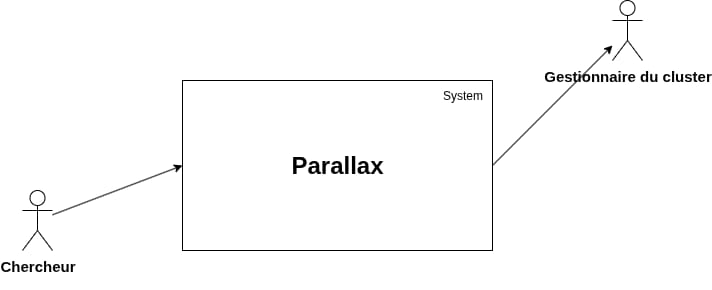
\includegraphics[width=1\textwidth]{images/parallax - diagramme de context.jpeg}
    \caption{Diagramme de Contexte}
    \label{fig:diagramme_contexte}
\end{figure}

\textbf{Exigences fonctionnelles :}
\begin{itemize}
    \item Soumission et exécution distribuée de tâches de calcul (Chercheur).
    \item Import et annotation de programmes via interface CLI (Chercheur).
    \item Consultation des résultats d'exécution avec détails (durée, date) (Chercheur).
    \item Supervision en temps réel de l'état des nœuds via interface Web (Gestionnaire de cluster).
    \item Gestion dynamique du cluster : ajout et retrait de machines (Gestionnaire de cluster).
\end{itemize}

\textbf{Exigences non fonctionnelles :}
\begin{itemize}
    \item Résilience aux pannes : détection automatique et réaffectation des tâches, y compris en cas de surcharge d'un nœud.
    \item Transparence pour le développeur : parallélisation via annotations sans gestion manuelle du réseau.
    \item Légèreté : adaptation aux petits clusters hétérogènes à ressources modestes.
    \item Performance : optimisation de la distribution des tâches en fonction d'un score pondéré des nœuds (CPU, RAM, latence, fréquence), et prise en compte de la latence réseau afin de minimiser les temps de communication entre les machines.
\end{itemize}

\subsection{Diagramme de cas d'utilisation}

Le domaine du calcul distribué académique présente six exigences fondamentales. Le système doit fournir de la puissance de calcul pour les simulations et l'entraînement de modèles d'intelligence artificielle (ED-1). Il doit réduire les coûts d'infrastructure en proposant une alternative aux plateformes cloud distantes (ED-2). Il doit s'affranchir de la dépendance à une connexion Internet souvent instable dans le contexte camerounais (ED-3). Il doit permettre la mutualisation des machines existantes sous-utilisées sur le campus (ED-4). Il doit offrir une soumission de programmes sans expertise réseau, via un mécanisme d'annotations (ED-5). Enfin, il doit assurer la supervision et la maintenance continues du cluster par un administrateur (ED-6).

\begin{figure}[H]
    \centering
    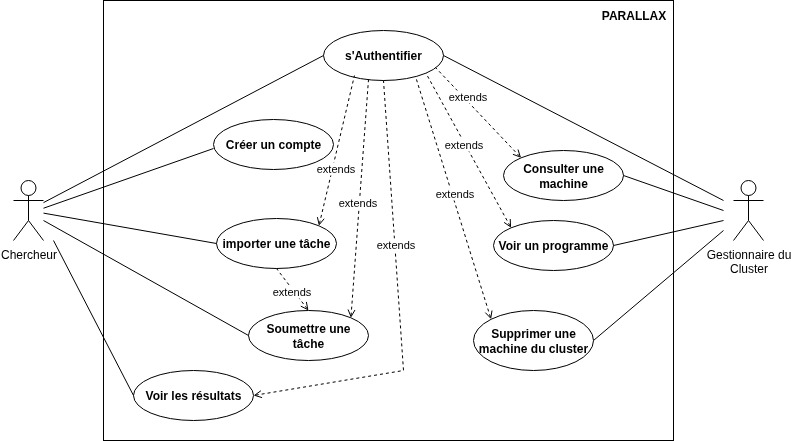
\includegraphics[width=\textwidth,height=\textheight,keepaspectratio]{images/Diagramme UC.jpg.jpeg}
    \caption{Diagramme de cas d'utilisation}
    \label{fig:use_case}
\end{figure}

Le cas d'utilisation « S'authentifier » constitue le point d'entrée commun. Les cas « Créer un compte », « Importer une tâche », « Soumettre une tâche » et « Voir les résultats » concernent le Chercheur. Les cas « Consulter une machine », « Voir un programme » et « Supprimer une machine du cluster » concernent le Gestionnaire du cluster.

\clearpage

\begin{table}[H]
\centering
\renewcommand{\arraystretch}{1.3}
\begin{tabular}{|p{4cm}|p{11cm}|}
\hline
\textbf{Objectif} & Accéder aux fonctionnalités du système \\
\hline
\textbf{Acteur(s)} & Chercheur, Gestionnaire du cluster \\
\hline
\textbf{Pré-condition} & Aucune \\
\hline
\textbf{Scénario nominal} &
\begin{enumerate}
    \item L'acteur entre ses informations d'identification dans le système.
    \item Le système vérifie l'exactitude des informations.
    \item Les informations sont correctes, le système accorde l'accès aux fonctionnalités correspondantes au statut de l'utilisateur.
\end{enumerate} \\
\hline
\textbf{Scénarios alternatifs} &
\begin{itemize}
    \item \textbf{A1 : Erreur de saisie} — Le système informe l'utilisateur et demande de nouvelles informations.
    \item \textbf{A2 : Erreur de connexion à la base de données} — Le système renvoie un message d'erreur.
\end{itemize} \\
\hline
\textbf{Post-condition} & Accès aux fonctionnalités liées au statut de l'utilisateur \\
\hline
\end{tabular}
\caption{Cas d'utilisation : Authentification}
\label{tab:authentification}
\end{table}

\begin{table}[H]
\centering
\renewcommand{\arraystretch}{1.3}
\begin{tabular}{|p{4cm}|p{11cm}|}
\hline
\textbf{Objectif} & Créer un compte utilisateur \\
\hline
\textbf{Acteur(s)} & Chercheur \\
\hline
\textbf{Pré-condition} & Être authentifié \\
\hline
\textbf{Scénario nominal} &
\begin{enumerate}
    \item L'acteur entre ses informations dans le formulaire et le soumet au système.
    \item Le système vérifie l'exactitude des informations.
    \item Le système sauvegarde les informations et renvoie un message de succès.
\end{enumerate} \\
\hline
\textbf{Scénarios alternatifs} &
\begin{itemize}
    \item \textbf{A1 : Erreur de saisie} — Le système demande à l'utilisateur de ressaisir ses informations.
    \item \textbf{A2 : Erreur de connexion à la base de données} — Le système renvoie un message d'erreur.
\end{itemize} \\
\hline
\textbf{Post-condition} & Création du compte utilisateur \\
\hline
\end{tabular}
\caption{Cas d'utilisation : Création de compte}
\label{tab:create_account}
\end{table}

\begin{table}[H]
\centering
\renewcommand{\arraystretch}{1.3}
\begin{tabular}{|p{4cm}|p{11cm}|}
\hline
\textbf{Objectif} & Importer une tâche annotée \\
\hline
\textbf{Acteur(s)} & Chercheur \\
\hline
\textbf{Pré-condition} & Être authentifié \\
\hline
\textbf{Scénario nominal} &
\begin{enumerate}
    \item L'utilisateur clique sur l'option d'importation d'une tâche.
    \item Le système lui permet de sélectionner le dossier ou fichier annoté via un sélecteur de ressources.
    \item L'utilisateur sélectionne et valide.
    \item La tâche est enregistrée dans le système.
\end{enumerate} \\
\hline
\textbf{Scénarios alternatifs} &
\begin{itemize}
    \item \textbf{A1 : Document invalide} — Le système annule l'importation et renvoie un message d'erreur.
\end{itemize} \\
\hline
\textbf{Post-condition} & Dossier / fichier importé dans le système \\
\hline
\end{tabular}
\caption{Cas d'utilisation : Importation d'une tâche}
\label{tab:import_task}
\end{table}

\begin{table}[H]
\centering
\renewcommand{\arraystretch}{1.3}
\begin{tabular}{|p{4cm}|p{11cm}|}
\hline
\textbf{Objectif} & Soumettre une tâche pour son exécution \\
\hline
\textbf{Acteur(s)} & Chercheur \\
\hline
\textbf{Pré-condition} & La tâche a été importée et le chercheur est authentifié \\
\hline
\textbf{Scénario nominal} &
\begin{enumerate}
    \item L'utilisateur sélectionne la tâche à soumettre et valide.
    \item Le Master, grâce aux annotations, découpe et distribue la tâche à exécuter.
    \item Les Workers exécutent la tâche et renvoient les résultats au Master pour recomposition.
    \item Le Master recompose et renvoie le résultat à l'utilisateur.
\end{enumerate} \\
\hline
\textbf{Scénarios alternatifs} &
\begin{itemize}
    \item \textbf{A1 : Erreur de connexion} — Un message d'erreur de connexion est renvoyé à l'utilisateur.
    \item \textbf{A2 : Dossier/fichier mal annoté} — Le système renvoie un message d'erreur d'annotation.
\end{itemize} \\
\hline
\textbf{Post-condition} & Le résultat de l'exécution est renvoyé à l'utilisateur \\
\hline
\end{tabular}
\caption{Cas d'utilisation : Soumission d'une tâche}
\label{tab:submit_task}
\end{table}

\begin{table}[H]
\centering
\renewcommand{\arraystretch}{1.3}
\begin{tabular}{|p{4cm}|p{11cm}|}
\hline
\textbf{Objectif} & Permettre à l'utilisateur de consulter les résultats de ses tâches exécutées \\
\hline
\textbf{Acteur(s)} & Chercheur \\
\hline
\textbf{Pré-condition} & Être authentifié \\
\hline
\textbf{Scénario nominal} &
\begin{enumerate}
    \item L'utilisateur sélectionne le menu des résultats.
    \item Le système affiche les résultats et les détails d'exécution (durée, date, etc.).
\end{enumerate} \\
\hline
\textbf{Scénarios alternatifs} &
\begin{itemize}
    \item \textbf{A1 : Aucun résultat} — Le système affiche un message indiquant l'absence de résultats.
    \item \textbf{A2 : Erreur de récupération} — Un message d'erreur est renvoyé à l'utilisateur.
\end{itemize} \\
\hline
\textbf{Post-condition} & Les résultats sont affichés à l'utilisateur \\
\hline
\end{tabular}
\caption{Cas d'utilisation : Consultation des résultats}
\label{tab:view_results}
\end{table}

\begin{table}[H]
\centering
\renewcommand{\arraystretch}{1.3}
\begin{tabular}{|p{4cm}|p{11cm}|}
\hline
\textbf{Objectif} & Consulter l'état d'une machine du cluster \\
\hline
\textbf{Acteur(s)} & Gestionnaire du cluster \\
\hline
\textbf{Pré-condition} & Être authentifié \\
\hline
\textbf{Scénario nominal} &
\begin{enumerate}
    \item L'utilisateur sélectionne l'option de consultation des machines.
    \item Le système affiche la liste des machines du cluster.
    \item L'utilisateur sélectionne la machine souhaitée.
    \item Le système affiche les détails de la machine sélectionnée.
\end{enumerate} \\
\hline
\textbf{Scénarios alternatifs} &
\begin{itemize}
    \item \textbf{A1 : Machine indisponible} — Le système affiche un message d'erreur d'accessibilité.
    \item \textbf{A2 : Liste vide} — Le système indique qu'aucune machine n'est disponible.
\end{itemize} \\
\hline
\textbf{Post-condition} & Les détails de la machine sont affichés \\
\hline
\end{tabular}
\caption{Cas d'utilisation : Consultation d'une machine}
\label{tab:view_machine}
\end{table}

\begin{table}[H]
\centering
\renewcommand{\arraystretch}{1.3}
\begin{tabular}{|p{4cm}|p{11cm}|}
\hline
\textbf{Objectif} & Déconnecter une machine du cluster \\
\hline
\textbf{Acteur(s)} & Gestionnaire du cluster \\
\hline
\textbf{Pré-condition} & Être authentifié \\
\hline
\textbf{Scénario nominal} &
\begin{enumerate}
    \item L'utilisateur sélectionne la machine à arrêter dans la liste.
    \item L'utilisateur déclenche la commande d'arrêt distant.
    \item Le système demande à l'agent sur la machine d'exécuter la commande d'arrêt.
    \item L'état de la machine est mis à jour sur l'interface pour confirmer l'arrêt.
\end{enumerate} \\
\hline
\textbf{Scénarios alternatifs} &
\begin{itemize}
    \item \textbf{A1 : Échec de communication} — Le système affiche un message d'échec et propose de réessayer.
    \item \textbf{A2 : Refus de confirmation} — L'utilisateur annule, la procédure est abandonnée sans modification.
    \item \textbf{A3 : Machine en cours d'exécution critique} — Le système demande une confirmation supplémentaire ou bloque l'action.
\end{itemize} \\
\hline
\textbf{Post-condition} & La machine est arrêtée (déconnectée du cluster) \\
\hline
\end{tabular}
\caption{Cas d'utilisation : Suppression d'une machine du cluster}
\label{tab:delete_machine}
\end{table}

\begin{table}[H]
\centering
\renewcommand{\arraystretch}{1.3}
\begin{tabular}{|p{4cm}|p{11cm}|}
\hline
\textbf{Objectif} & Voir en temps réel l'état d'un programme en cours d'exécution \\
\hline
\textbf{Acteur(s)} & Gestionnaire du cluster \\
\hline
\textbf{Pré-condition} & Être authentifié \\
\hline
\textbf{Scénario nominal} &
\begin{enumerate}
    \item L'utilisateur sélectionne l'option de consultation des tâches en cours.
    \item Le système affiche la liste des tâches actives.
    \item L'utilisateur sélectionne la tâche souhaitée.
    \item Le système affiche les détails d'exécution (machines impliquées, pourcentage d'avancement, etc.).
\end{enumerate} \\
\hline
\textbf{Scénarios alternatifs} &
\begin{itemize}
    \item \textbf{A1 : Aucune tâche en cours} — Le système affiche un message d'absence de tâches actives.
    \item \textbf{A2 : Erreur de récupération} — Le système affiche un message d'erreur et propose de réessayer.
\end{itemize} \\
\hline
\textbf{Post-condition} & Les détails d'exécution de la tâche sont affichés \\
\hline
\end{tabular}
\caption{Cas d'utilisation : Consultation d'un programme en cours d'exécution}
\label{tab:view_program}
\end{table}

\subsection{Identification des agents}

L'examen des cas d'utilisation révèle quatre entités autonomes aux responsabilités distinctes.

\begin{table}[H]
\centering
\renewcommand{\arraystretch}{1.3}
\begin{tabular}{|p{4.5cm}|p{5.5cm}|c|}
\hline
\textbf{Groupement fonctionnel} & \textbf{Justification d'autonomie} & \textbf{Agent} \\
\hline
Accueillir les soumissions de code, exposer l'interface de supervision et relayer les programmes vers le Master & Point d'entrée autonome, indépendant du flux de calcul & \texttt{<<Agent>>} Réceptionniste \\
\hline
Gérer la réception, décomposition et recomposition des calculs & Vision globale du calcul et des ressources & \texttt{<<Agent>>} Master \\
\hline
Exécuter des calculs locaux & Autonomie d'exécution, capacité de refus selon charge & \texttt{<<Agent>>} Worker \\
\hline
Superviser l'état du réseau et détecter les pannes & Observation indépendante du flux de calcul & \texttt{<<Agent>>} Contrôleur \\
\hline
\end{tabular}
\caption{Identification des agents}
\label{tab:identification_agents}
\end{table}

L'Agent Réceptionniste constitue le point d'entrée unique du système : il reçoit les soumissions de code des utilisateurs, les relaie au Master et expose une interface de supervision du cluster. L'Agent Master assume les fonctions de décomposition des calculs, d'orchestration de leur répartition et d'agrégation des résultats. L'Agent Worker est responsable de l'exécution locale des sous-calculs qui lui sont confiés ; chaque machine physique héberge une instance de cet agent. L'Agent Contrôleur maintient une vision globale de l'état du système et détecte les anomalies.

\subsection{Identification des rôles}

\begin{table}[H]
\centering
\renewcommand{\arraystretch}{1.3}
\begin{tabular}{|l|l|l|}
\hline
\textbf{Agent} & \textbf{Rôle} & \textbf{Responsabilité observable} \\
\hline
\multirow{2}{*}{Réceptionniste} & Passerelle utilisateur & Recevoir les soumissions de code et les relayer au Master \\
 & Superviseur HTTP & Exposer l'état du cluster et les journaux d'exécution via une API web \\
\hline
\multirow{4}{*}{Master} & Réceptionniste & Accueillir et valider les programmes soumis \\
 & Générateur & Transformer un programme annoté en unités distribuables \\
 & Orchestrateur & Décider de l'allocation des sous-tâches aux Workers \\
 & Synthétiseur & Combiner les résultats partiels en résultat final \\
\hline
\multirow{2}{*}{Worker} & Exécuteur & Réaliser le calcul local et signaler la terminaison \\
 & Signaleur d'état & Émettre périodiquement les métriques de charge \\
\hline
\multirow{2}{*}{Contrôleur} & Observateur & Collecter et centraliser les informations d'état \\
 & Détecteur de panne & Identifier les anomalies et alerter les agents concernés \\
\hline
\end{tabular}
\caption{Identification des rôles}
\label{tab:identification_roles}
\end{table}

\subsection{Identification du SMA}

\subsubsection{Organisation}

L'organisation est hiérarchique fonctionnelle sans contrôle autoritaire. Le Master coordine mais ne commande pas : il propose des sous-calculs aux Workers qui conservent le droit de refuser. Le Contrôleur observe sans intervenir dans le flux de calcul. Cette organisation émerge des dépendances naturelles : le Master dépend des Workers pour l'exécution, les Workers dépendent du Master pour l'obtention des tâches, et le Master dépend du Contrôleur pour une vision fiable des ressources.

Tous les agents partagent le même objectif global — l'exécution efficace des calculs — mais avec des points de vue partiels. Le Master a une vue globale du calcul mais pas de l'état réseau en temps réel. Le Worker a une vue locale de sa charge mais ignore la charge des autres. Le Contrôleur a une vue globale de la présence des nœuds mais ignore la sémantique des calculs.

\subsubsection{Environnement}

L'environnement est un réseau local académique aux caractéristiques contraignantes. La couche physique comprend un switch Ethernet à cinq ports et six câbles RJ45 sertis manuellement, limitant l'extension à six nœuds. La latence est faible mais la bande passante est modeste. L'absence de redondance réseau fait du switch un point de défaillance unique.

La couche informatique est hétérogène : trois machines DELL sous Ubuntu Server 18.04 avec des processeurs Intel Core 2 Duo et des mémoires de 2 à 4 Go ; trois thin clients Wyse sous Windows CE avec 32 à 64 Mo de RAM et des processeurs de 533 MHz à 1 GHz.

Chaque agent perçoit son environnement via les métriques locales de sa machine ($LOAD_v$, $NET_v$) et via les messages reçus des autres agents. Il agit sur l'environnement en envoyant des messages TCP, en exécutant des calculs localement ou en modifiant l'état du cluster via les mécanismes d'élection et d'enregistrement.

L'environnement est dynamique : ajout et retrait volontaires par le Gestionnaire, pannes et surcharges imprévues, connectivité Internet externe instable rendant le cluster autonome une nécessité.

\subsubsection{Séquences système}

\begin{figure}[H]
    \centering
    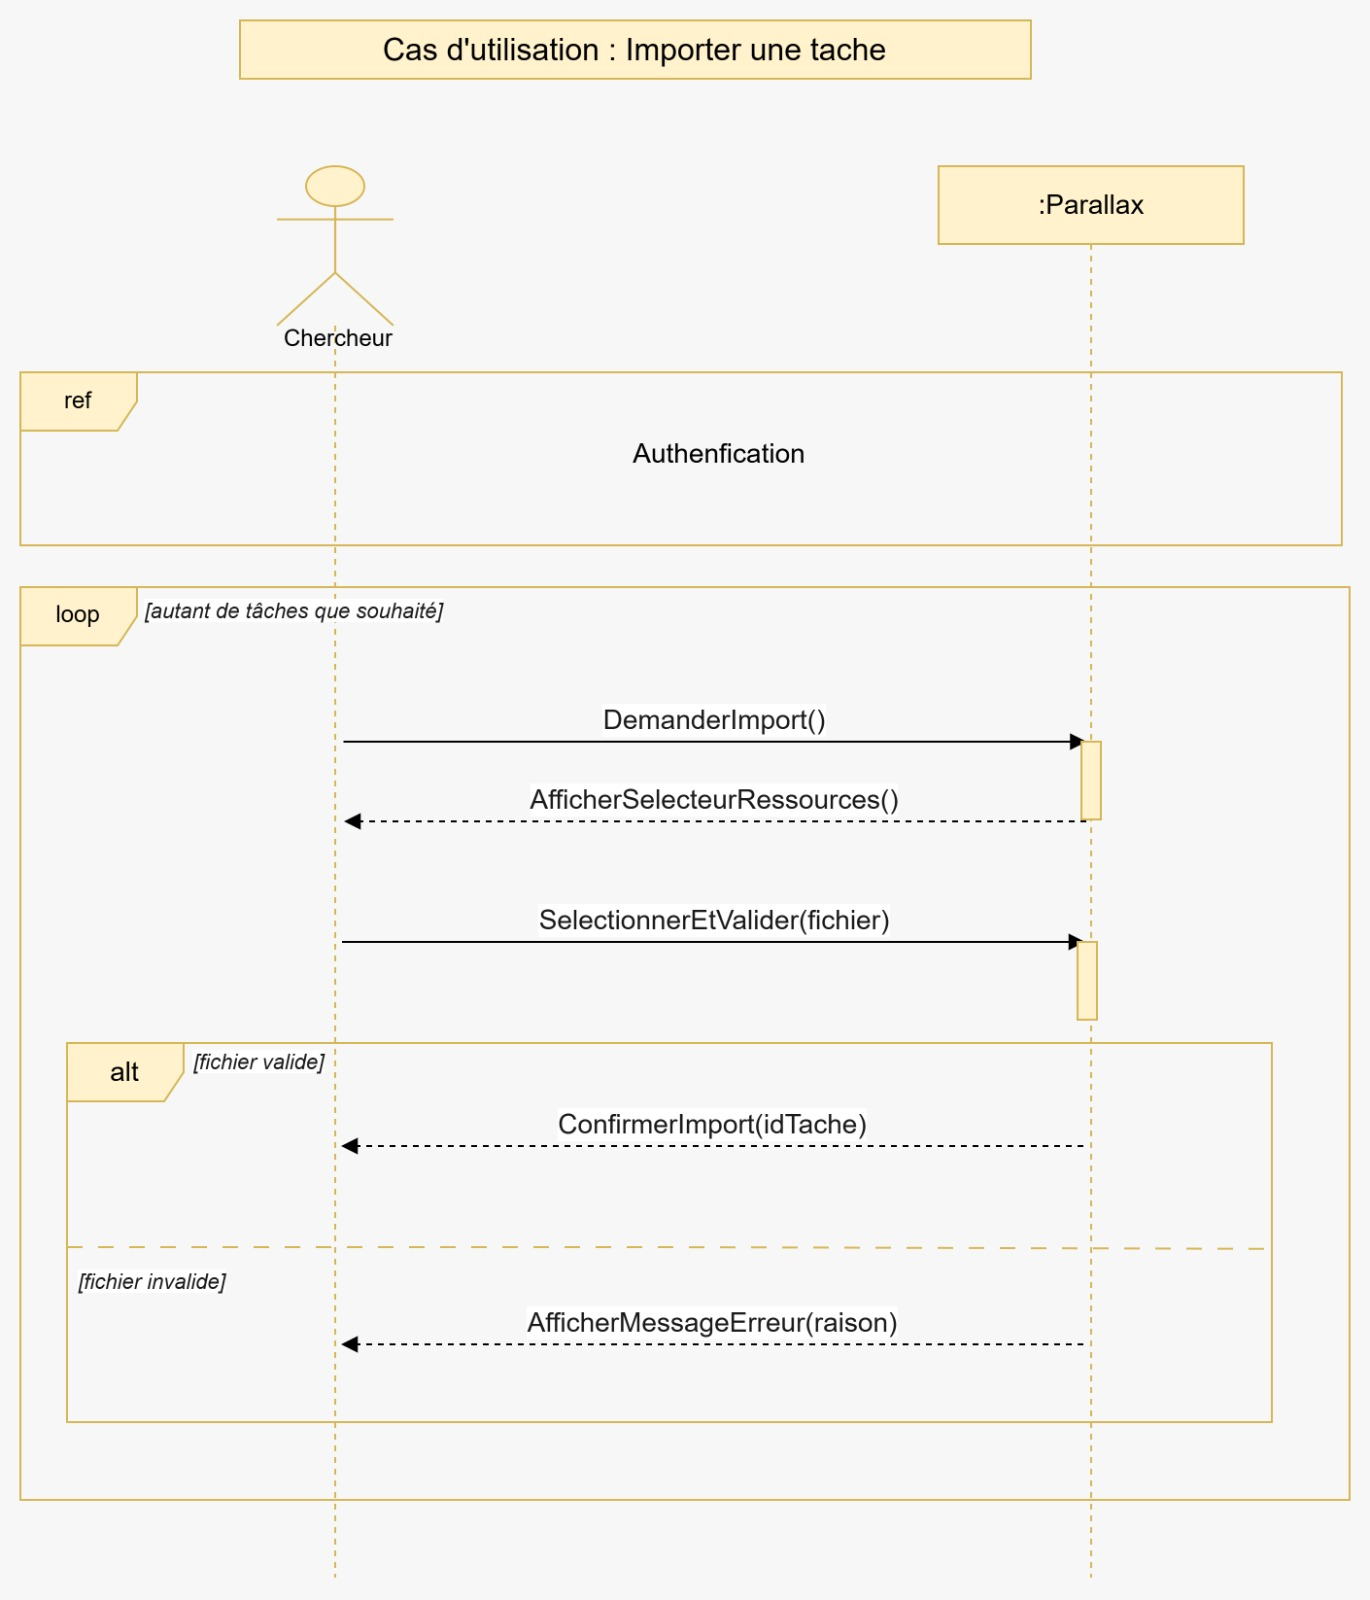
\includegraphics[width=1\textwidth]{images/diagramme de sequences - importer une tache - parallax .jpeg}
    \caption{Diagramme de séquences système — Importer une tâche}
    \label{fig:seq_import}
\end{figure}

\begin{figure}[H]
    \centering
    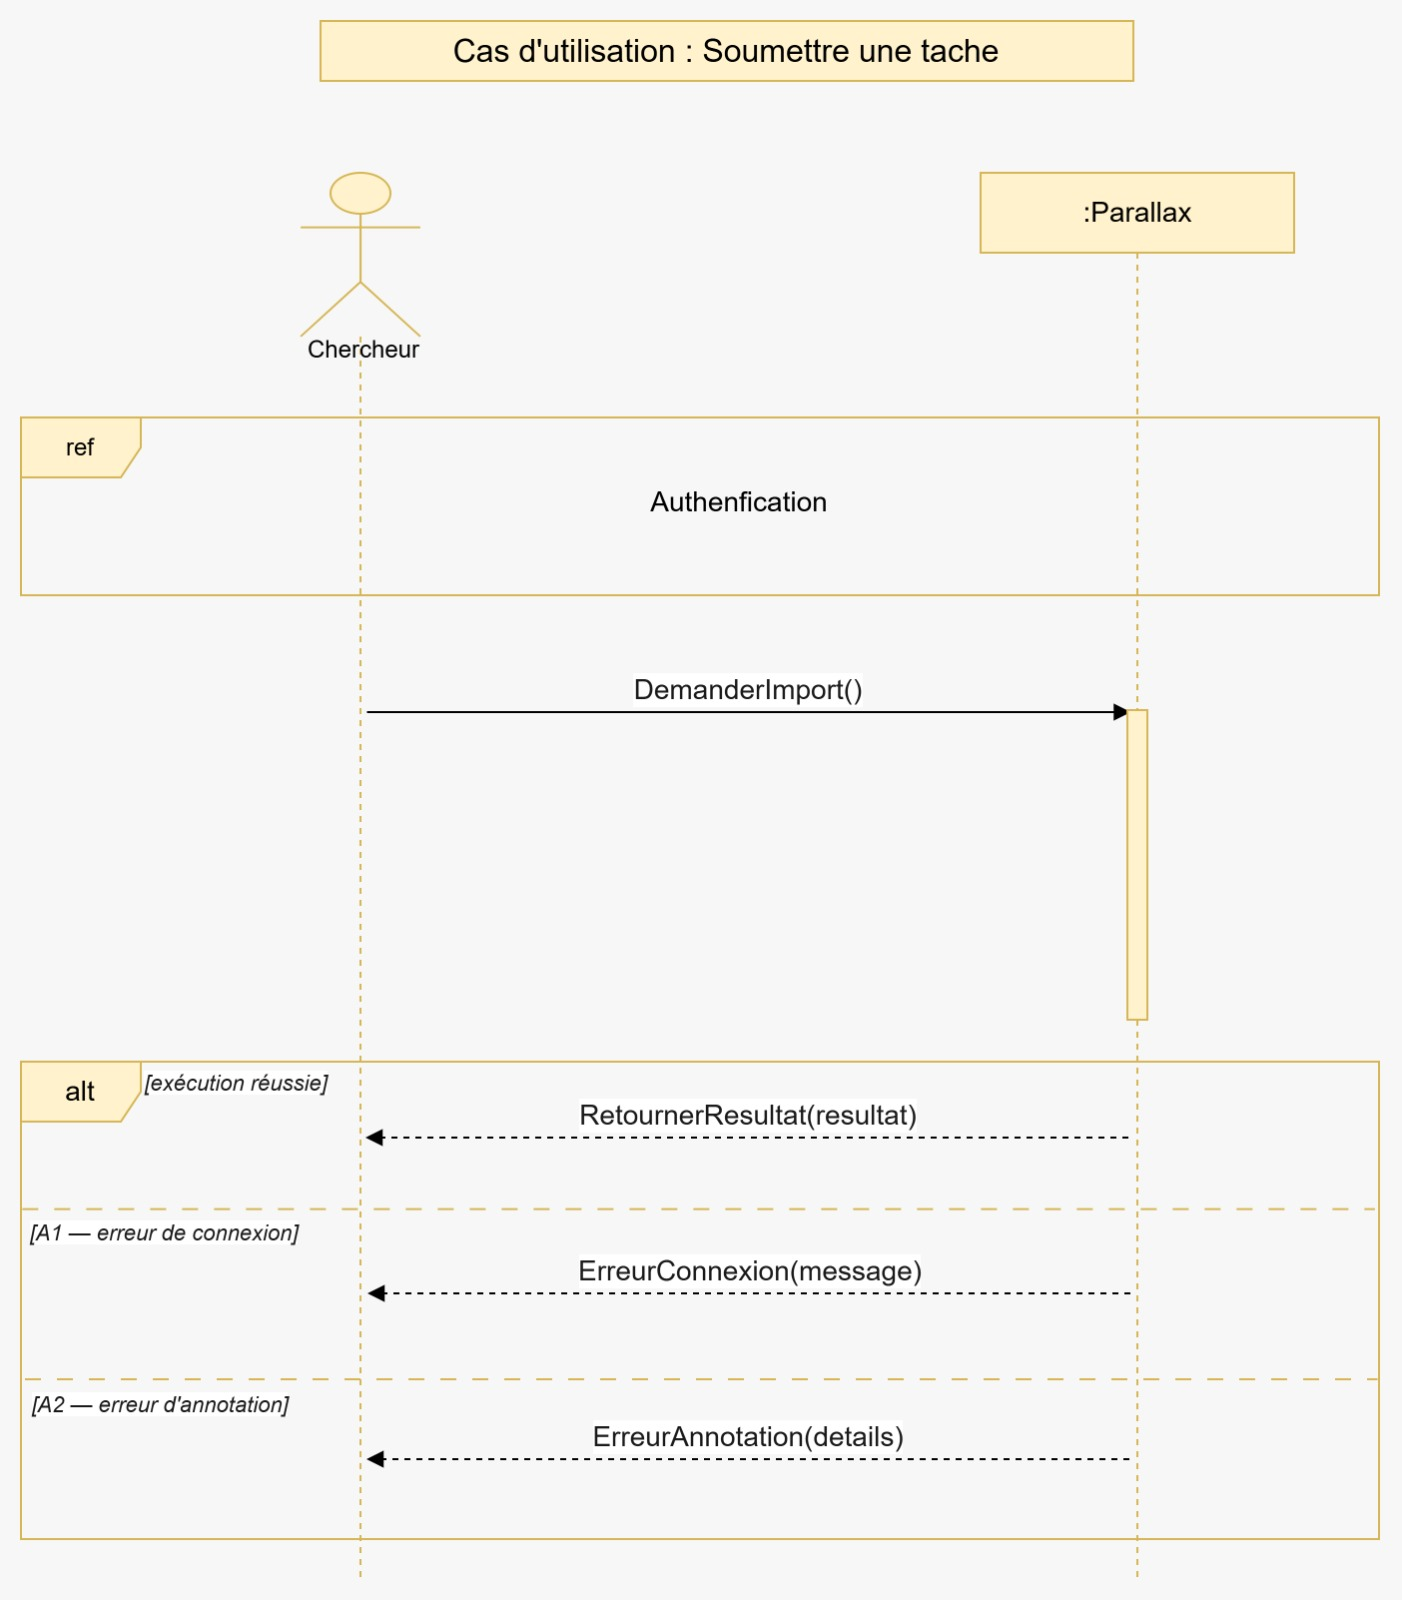
\includegraphics[width=1\textwidth]{images/diagramme de sequence - soumettre une tache- parallax.jpeg}
    \caption{Diagramme de séquences système — Soumettre une tâche}
    \label{fig:seq_soumettre}
\end{figure}

\begin{figure}[H]
    \centering
    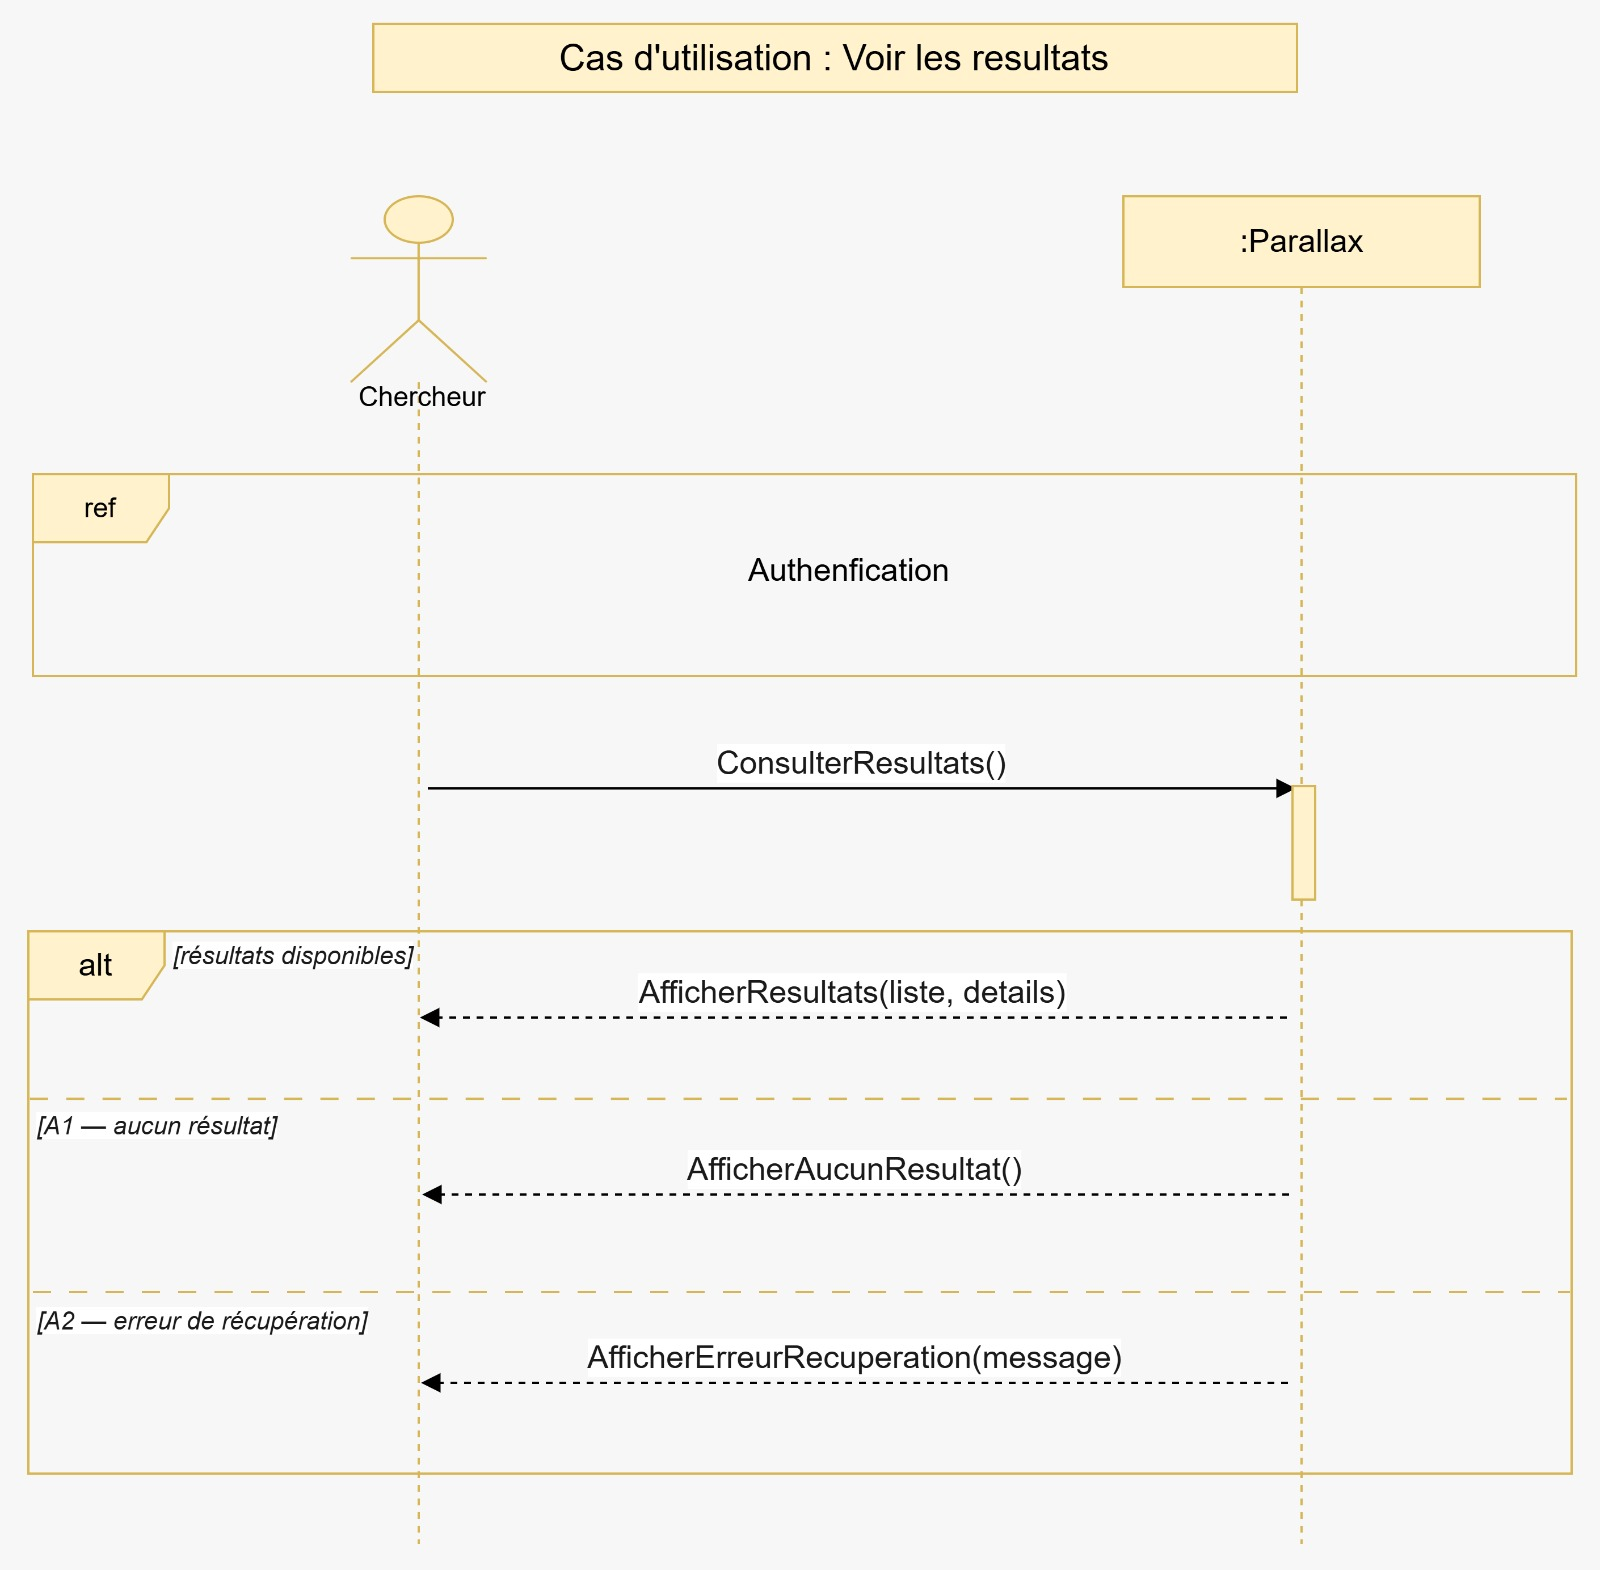
\includegraphics[width=1\textwidth]{images/sequence systeme - voir les resultats.jpeg}
    \caption{Diagramme de séquences système — Voir les résultats}
    \label{fig:seq_resultats}
\end{figure}

\begin{figure}[H]
    \centering
    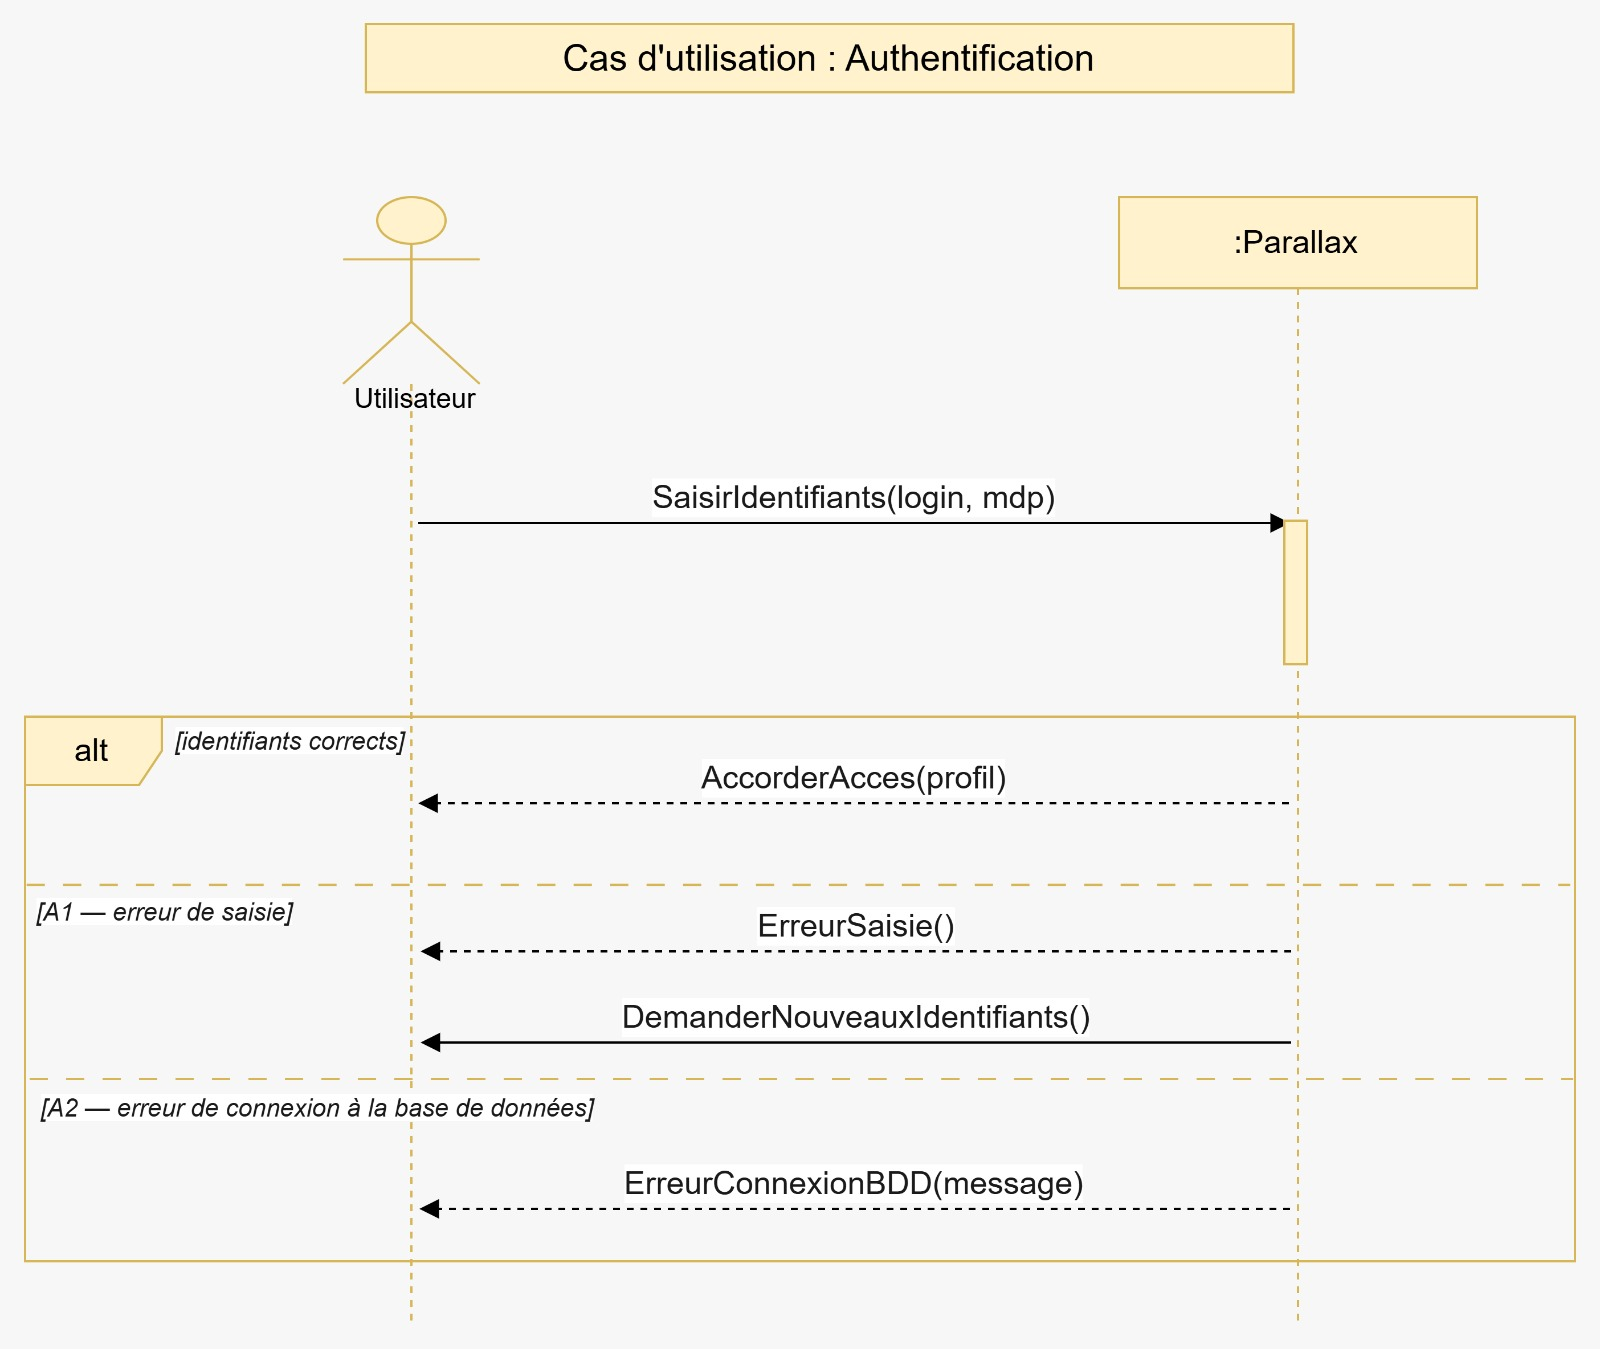
\includegraphics[width=1\textwidth]{images/diagramme de sequences systeme - authhentification - parallax.jpeg}
    \caption{Diagramme de séquences système — Authentification}
    \label{fig:seq_auth}
\end{figure}

\begin{figure}[H]
    \centering
    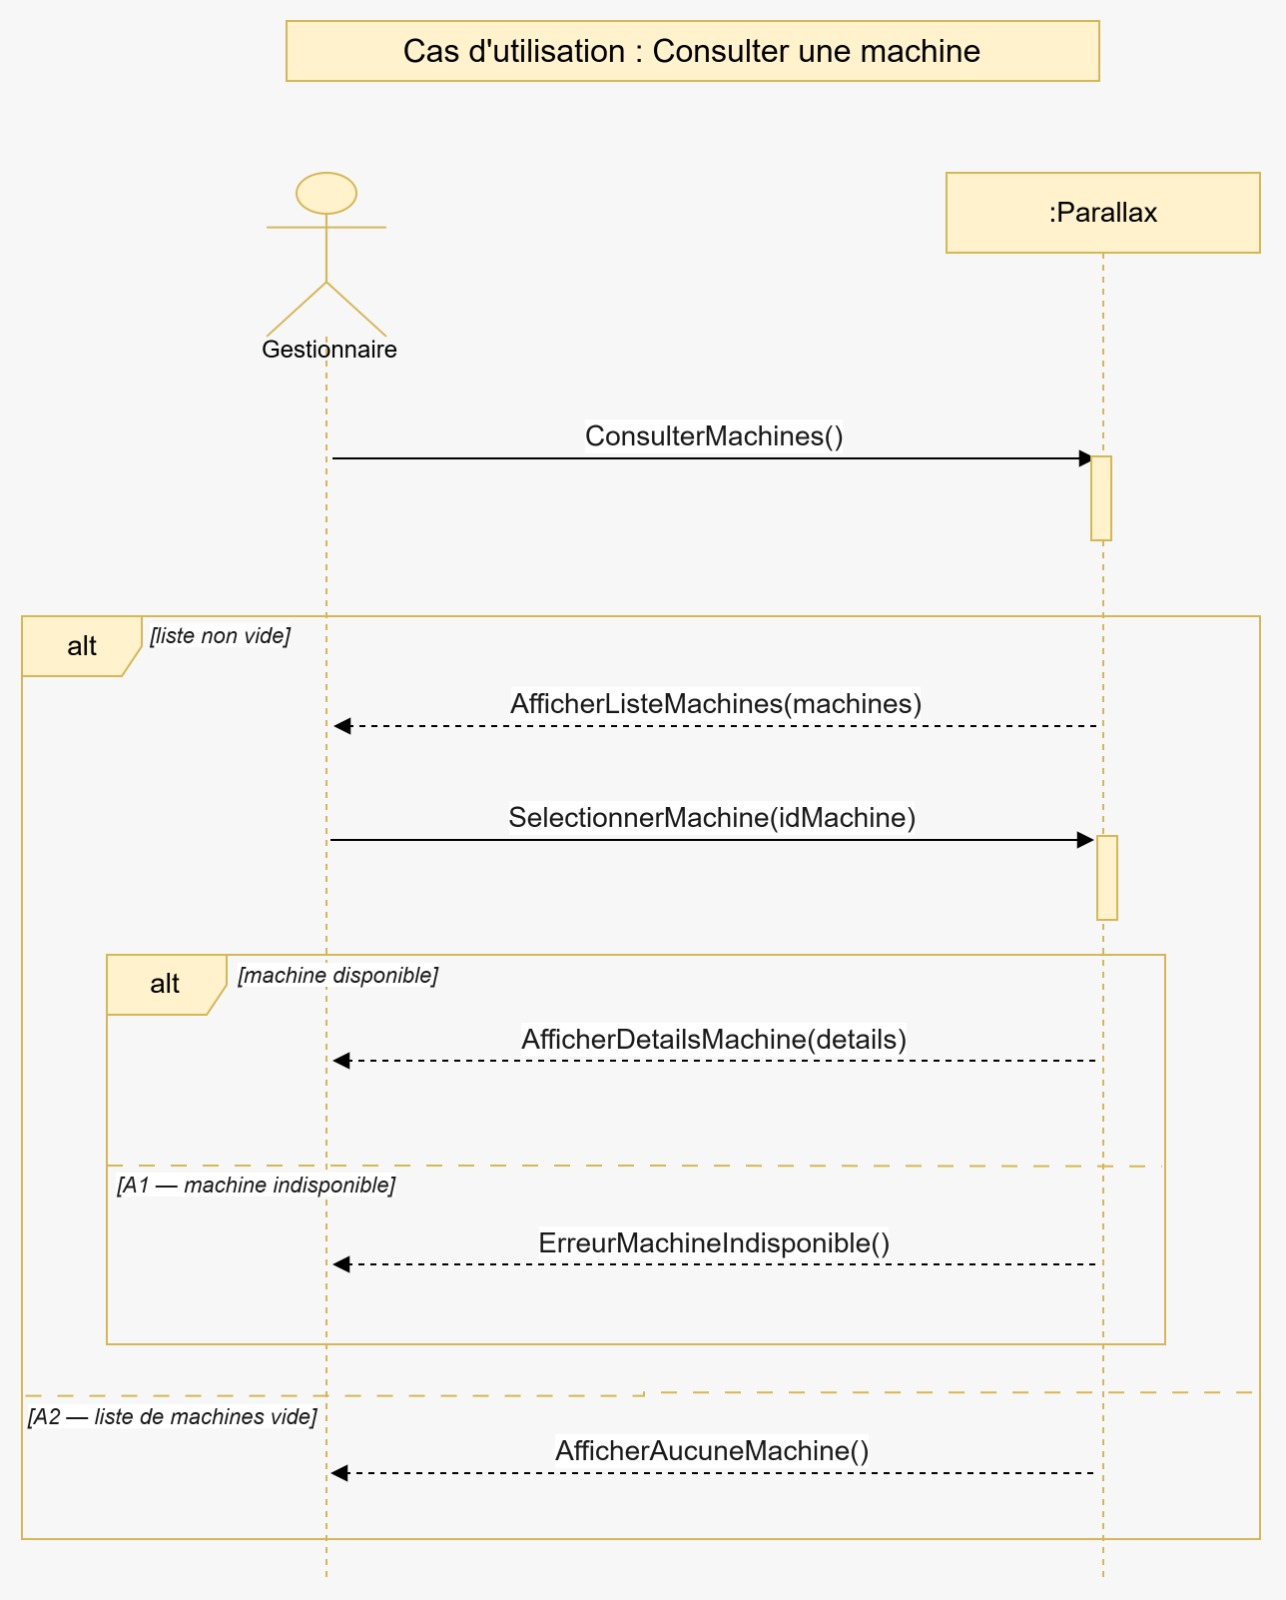
\includegraphics[width=1\textwidth]{images/sequence systeme - consulter une machine.jpeg}
    \caption{Diagramme de séquences système — Consulter une machine}
    \label{fig:seq_machine}
\end{figure}

% ==============================================================================
\section{Conception}
% ==============================================================================

La conception du système traduit les éléments identifiés en phase d'analyse en une architecture opérationnelle. Elle définit la structure des agents, leurs comportements, les protocoles de communication et les mécanismes de coordination distribuée assurant l'exécution des calculs dans un cluster hétérogène.

\subsection{Architecture du SMA}

L'architecture de SMA\_PARALLAX est hiérarchique fonctionnelle à trois niveaux :

\begin{itemize}
    \item \textbf{Niveau supervision} (Contrôleur) : maintient une vue globale cohérente, détecte les pannes, gère l'élection.
    \item \textbf{Niveau coordination} (Master) : reçoit les calculs, décompose, distribue et agrège les résultats.
    \item \textbf{Niveau exécution} (Workers) : réalise les sous-calculs de manière autonome et signale leur état.
\end{itemize}

Cette architecture hybride combine la réactivité du niveau inférieur (heartbeat, détection rapide) et la délibération du niveau supérieur (planification de la distribution, élection du remplaçant).

\begin{figure}[H]
    \centering
    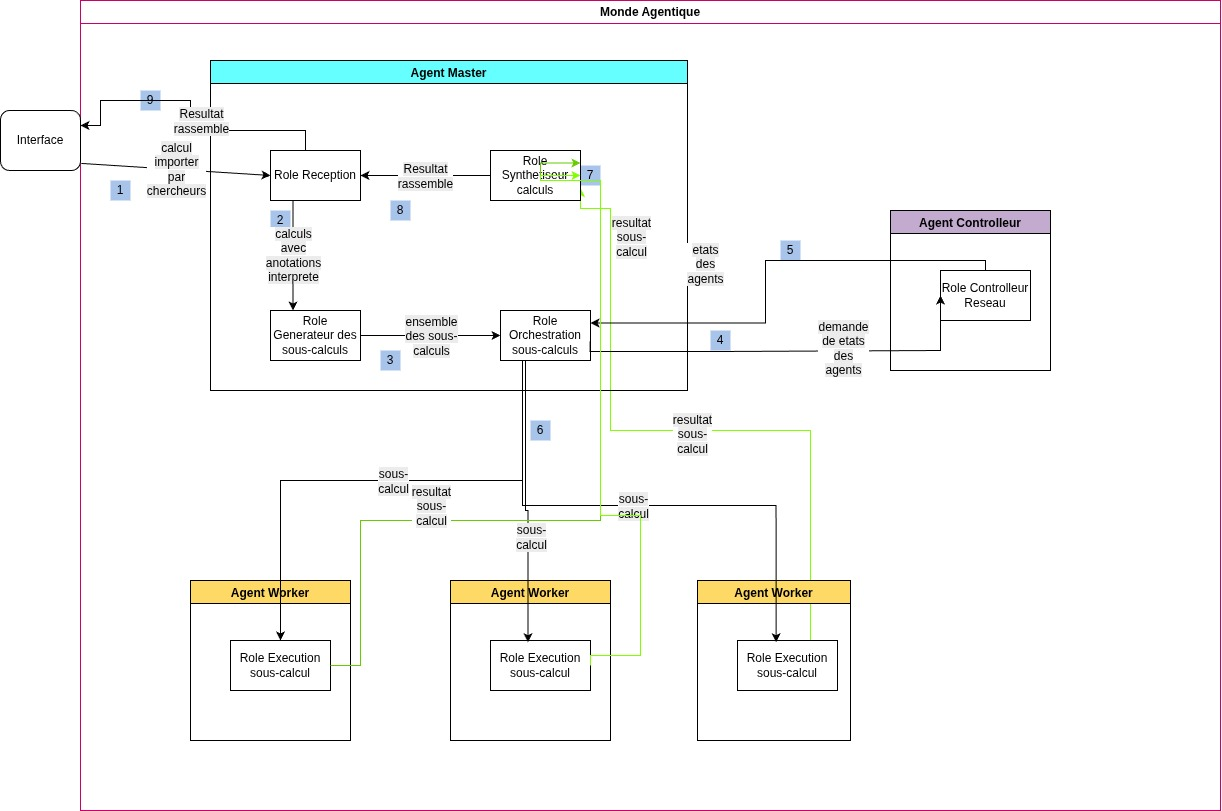
\includegraphics[width=1.0\linewidth]{Architecture_agentique (2).jpg}
    \caption{Architecture agentique de SMA\_PARALLAX}
    \label{fig:architecture_agentique}
\end{figure}

\subsection{Structure de l'agent et du SMA}

\subsubsection{Modélisation physique d'un nœud}

Chaque machine $v \in V_M$ est caractérisée par un vecteur d'état :

\[
X_v =
\begin{bmatrix}
ID_v \\ NET_v \\ COMPUTE_v \\ MEMORY_v \\ STORAGE_v \\
LOAD_v \\ RELIABILITY_v \\ STATE_v \\ SECURITY_v
\end{bmatrix}
\]

\begin{itemize}
    \item[*] $ID_v = (\text{uuid}, \text{role}, \text{region})$ : identité unique, rôle et localisation.
    \item[*] $NET_v = (\text{ip}, \text{latency}, \text{bandwidth}_{in}, \text{bandwidth}_{out}, \text{jitter}, \text{loss})$ : performances réseau.
    \item[*] $COMPUTE_v = (\text{cpucores}, \text{cpufreq}, \text{gpu}, \text{flops})$ : capacités de calcul.
    \item[*] $MEMORY_v = (\text{ram}, \text{mem\_bandwidth})$ : ressources mémoire.
    \item[*] $STORAGE_v = (\text{disk}, \text{io})$ : capacités de stockage.
    \item[*] $LOAD_v = (\text{cpuusage}, \text{ramusage}, \text{queue})$ : charge courante.
    \item[*] $STATE_v = (\text{status}, \text{availability})$ : état opérationnel.
    \item[*] $RELIABILITY_v = (\text{uptime}, \text{failurerate})$ : fiabilité.
    \item[*] $SECURITY_v = (\text{auth}, \text{trust})$ : sécurité et confiance.
\end{itemize}

\subsubsection{Modélisation mentale : architecture BDI des agents cognitifs}

Les agents Master et Contrôleur suivent une architecture BDI (Belief-Desire-Intention), fondée sur la théorie de l'action rationnelle de Michael Bratman telle que présentée dans le cours \cite{chapitre2}, qui structure leur état mental en trois composantes \cite{wooldridge} :

\begin{itemize}
    \item \textbf{Croyances ($B$)} : représentation informationnelle de l'état du monde. Le Master maintient des croyances sur l'état des Workers (charge, disponibilité) via le Contrôleur. Le Contrôleur maintient des croyances sur la présence et la santé de tous les nœuds via les heartbeats.
    \item \textbf{Désirs ($D$)} : états que l'agent souhaite atteindre. Le Master désire minimiser le temps global d'exécution des calculs. Le Contrôleur désire maximiser la disponibilité du cluster.
    \item \textbf{Intentions ($I$)} : engagements délibérés que l'agent poursuit activement. Le Master forme l'intention de distribuer les sous-calculs selon le score pondéré. Le Contrôleur forme l'intention de déclencher une élection lors d'une défaillance critique.
\end{itemize}

Par exemple, lorsque le Contrôleur envoie une alerte de panne d'un Worker en cours d'exécution, le Master révise ses croyances (ce Worker n'est plus disponible), met à jour ses intentions (réaffecter les tâches en cours de ce Worker) et planifie immédiatement leur redistribution vers les nœuds disponibles restants.

\textbf{\large Les agents Worker et Réceptionniste, de type réactif avec état, ne suivent pas le cycle BDI complet : ils maintiennent un état interne minimal (charge pour le Worker, coordonnées du Master/Contrôleur pour le Réceptionniste) et réagissent par des règles condition-action sans délibération symbolique.}

\subsubsection{Typologie des agents de SMA\_PARALLAX}

\begin{table}[H]
\centering
\renewcommand{\arraystretch}{1.5}
\begin{tabular}{|>{\bfseries}p{3cm}|p{3.2cm}|p{5.5cm}|p{3cm}|}
\hline
\textbf{Agent} & \textbf{Type} & \textbf{Justification} & \textbf{État interne} \\
\hline
AgentRéceptionniste & Réactif avec état \cite{chapitre2} & Perçoit les requêtes HTTP et les soumissions utilisateur, met en cache les programmes et journaux, réagit par transfert réseau conditionnel & UUID, IP du Contrôleur, IP du Master actif, cache des logs locaux \\
\hline
AgentWorker & Réactif avec état \cite{chapitre2} & Perçoit l'environnement via heartbeat, maintient un état interne (charge, file de tâches), réagit par règles condition-action sans délibération & $LOAD_v$, file des tâches en cours \\
\hline
AgentMaster & Cognitif orienté but \cite{chapitre2} & Représente symboliquement l'état du cluster, planifie la décomposition et la distribution selon un but de minimisation du temps global & Croyances sur le cluster, buts de répartition, intentions de distribution \\
\hline
AgentContrôleur & Cognitif orienté utilité \cite{chapitre2} & Évalue les configurations du cluster via une fonction d'utilité (fiabilité, cohérence de la vue globale) & Modèle social des nœuds, historique des pannes \\
\hline
\end{tabular}
\caption{Typologie des agents de SMA\_PARALLAX}
\label{tab:typologie_agents}
\end{table}

\subsubsection{Diagramme de classes}

\begin{figure}[H]
    \centering
    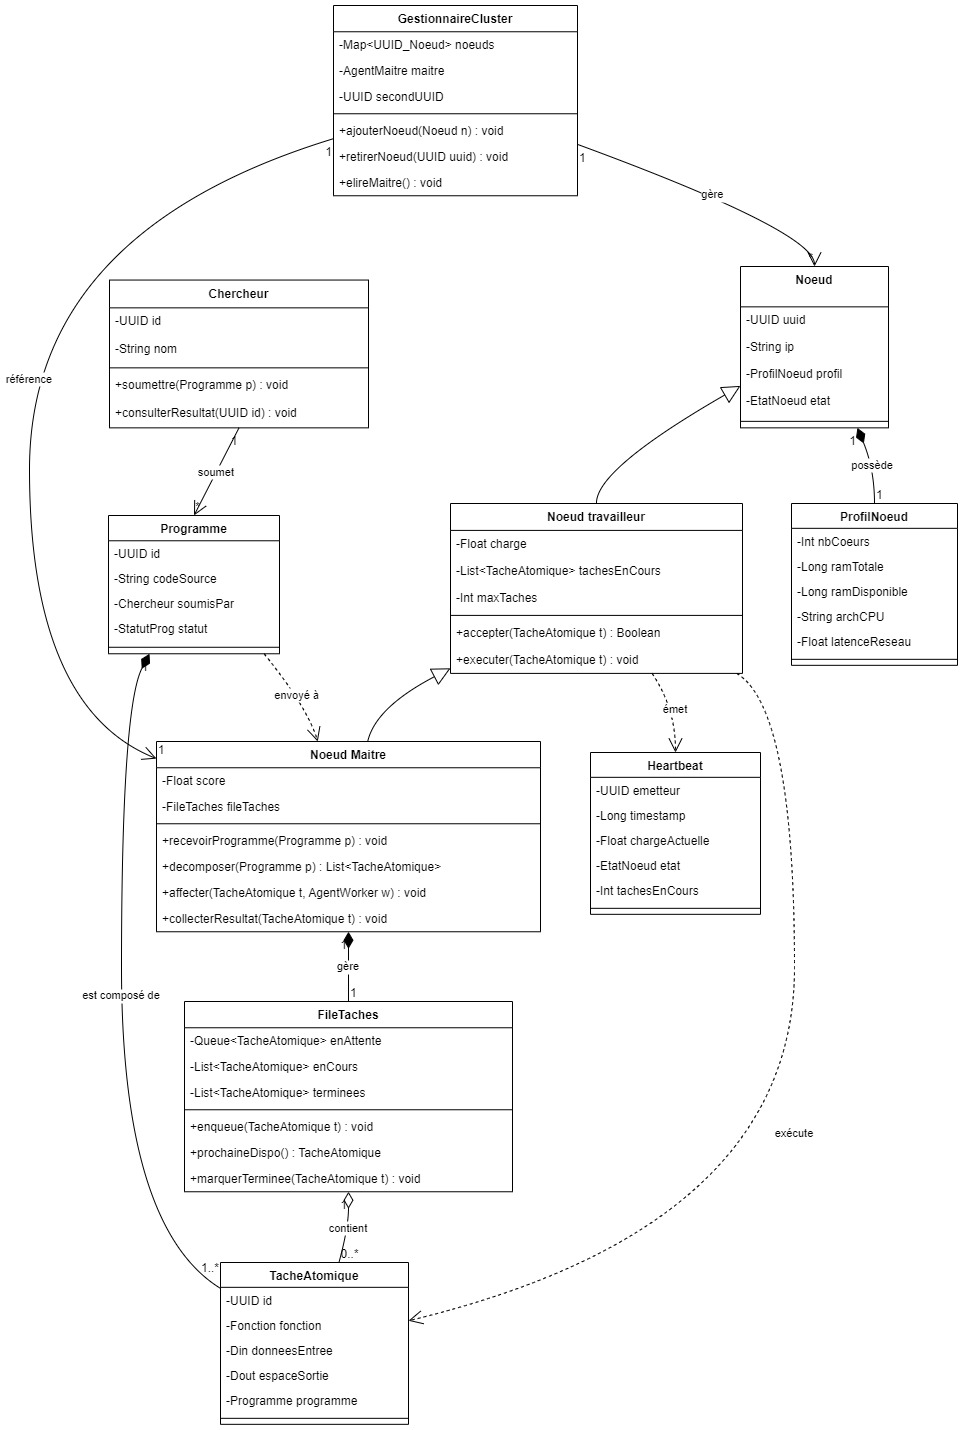
\includegraphics[width=1\textwidth]{images/parralax-classe technique.jpg}
    \caption{Diagramme de classes}
    \label{fig:classes}
\end{figure}

\subsubsection{Actions et événements du système}

\begin{table}[H]
\centering
\renewcommand{\arraystretch}{1.3}
\begin{tabular}{|c|p{3cm}|p{3.5cm}|p{3cm}|p{2cm}|p{2cm}|}
\hline
\textbf{N°} & \textbf{Action} & \textbf{Commentaire} & \textbf{Rôle} & \textbf{Entrée} & \textbf{Sortie} \\
\hline
1 & Réception des calculs & Prise en charge des requêtes & Réception (Master) & Requête utilisateur & Tâche globale \\
\hline
2 & Décomposition & Division en sous-calculs & Génération (Master) & Tâche globale & Sous-calculs \\
\hline
3 & Distribution & Allocation aux Workers & Orchestration (Master) & Sous-calculs + états & Tâches assignées \\
\hline
4 & Réception sous-calcul & Réception par le Worker & Exécution (Worker) & Sous-calcul & Tâche locale \\
\hline
5 & Exécution & Calcul effectif & Exécution (Worker) & Tâche locale & Résultat partiel \\
\hline
6 & Retour résultat & Envoi au Master & Exécution (Worker) & Résultat partiel & Résultat transmis \\
\hline
7 & Agrégation & Combinaison des résultats & Synthèse (Master) & Résultats partiels & Résultat final \\
\hline
8 & Observation & Surveillance ressources & Contrôle (Master) & États agents & Vue système \\
\hline
9 & Diffusion état Worker & Communication charge/dispo & Contrôle (Worker) & État local & Infos d'état \\
\hline
10 & Collecte états & Centralisation des infos & Contrôle (Contrôleur) & Infos d'état & BDD état \\
\hline
11 & Détection pannes & Identification anomalies & Contrôle (Contrôleur) & États système & Alertes \\
\hline
12 & Notification défaillance & Alerte au Master & Contrôle (Contrôleur) & Alertes & Notification \\
\hline
13 & Enregistrement nœud & Ajout au cluster & Contrôle (Contrôleur) & Infos nœud & Nœud enregistré \\
\hline
\end{tabular}
\caption{Table des actions de SMA\_PARALLAX}
\label{tab:actions}
\end{table}

\begin{table}[H]
\centering
\renewcommand{\arraystretch}{1.3}
\begin{tabular}{|c|p{4cm}|p{9cm}|}
\hline
\textbf{N°} & \textbf{Événement} & \textbf{Description} \\
\hline
E1 & Soumission de calcul & Un utilisateur soumet une requête via l'interface. Déclenche l'agent de réception. \\
\hline
E2 & Réception tâche globale & Le Master reçoit et valide la tâche. \\
\hline
E3 & Décomposition déclenchée & La tâche est transformée en sous-calculs. \\
\hline
E4 & Disponibilité des ressources & Les états des Workers orientent la planification. \\
\hline
E5 & Allocation des sous-calculs & Les sous-tâches sont assignées selon le score pondéré. \\
\hline
E6 & Réception sous-calcul & Un Worker reçoit une tâche à exécuter. \\
\hline
E7 & Début d'exécution & Le Worker commence le traitement. \\
\hline
E8 & Fin d'exécution & Le Worker produit un résultat partiel. \\
\hline
E9 & Envoi résultat partiel & Le résultat est transmis au Master. \\
\hline
E10 & Réception résultats partiels & Le Master collecte les résultats des Workers. \\
\hline
E11 & Agrégation & Les résultats partiels sont combinés. \\
\hline
E12 & Production résultat final & Le résultat est prêt à être renvoyé à l'utilisateur. \\
\hline
E13 & Diffusion état Worker & Les Workers envoient périodiquement leur état. \\
\hline
E14 & Collecte des états & Le Contrôleur centralise les informations. \\
\hline
E15 & Détection de défaillance & Une anomalie est détectée. \\
\hline
E16 & Notification de défaillance & Une alerte est envoyée au Master. \\
\hline
E17 & Enregistrement nouveau nœud & Un nouvel agent rejoint le système. \\
\hline
\end{tabular}
\caption{Table des événements de SMA\_PARALLAX}
\label{tab:events}
\end{table}

\subsection{Comportement des agents}

Le comportement des agents est régi par leurs états internes et les transitions déclenchées par les événements du système.

\begin{figure}[H]
    \centering
    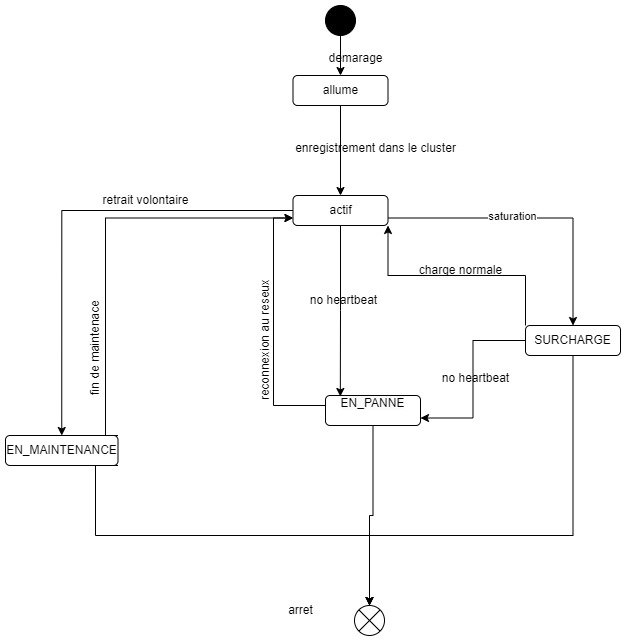
\includegraphics[width=1\textwidth]{images/parralax-etat d'un noeud.jpg}
    \caption{Diagramme d'état d'un nœud}
    \label{fig:etat_noeud}
\end{figure}

\begin{figure}[H]
    \centering
    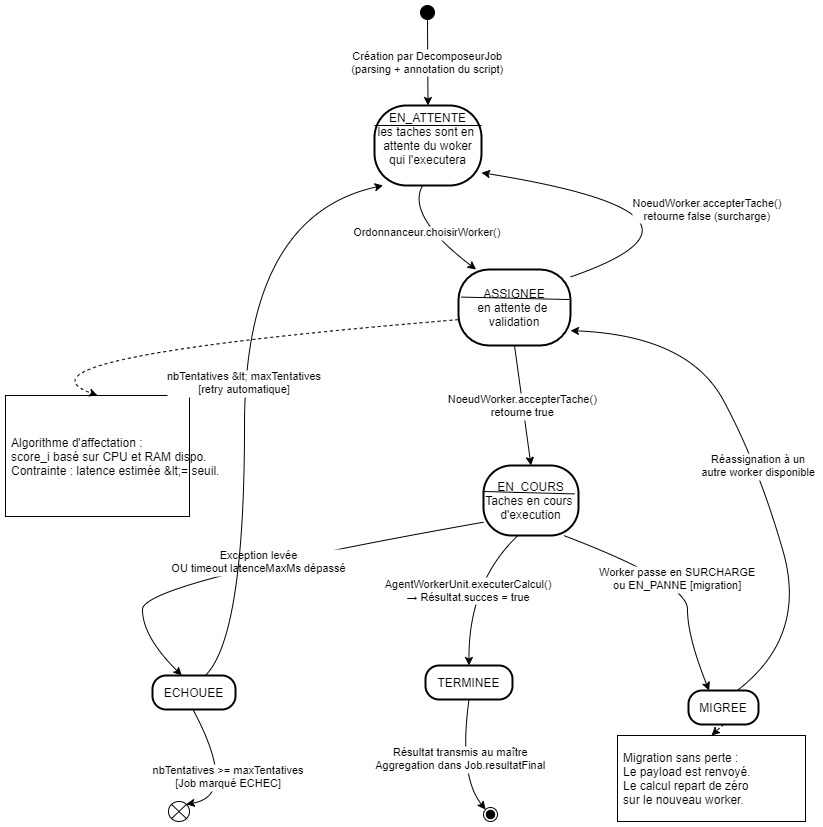
\includegraphics[width=1\textwidth]{images/parralax-etat d'une tache.jpg}
    \caption{Diagramme d'état d'une tâche}
    \label{fig:etat_tache}
\end{figure}

\begin{figure}[H]
    \centering
    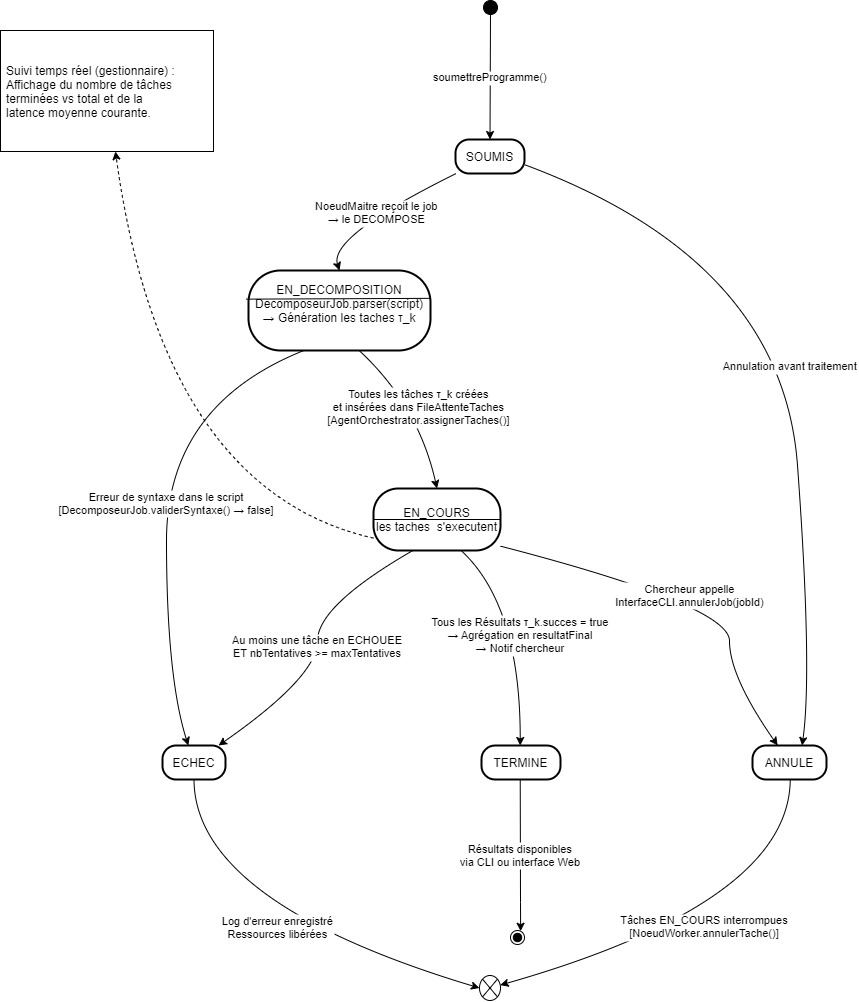
\includegraphics[width=1\textwidth]{images/parralax-etat d'un programme.jpg}
    \caption{Diagramme d'état d'un programme}
    \label{fig:etat_programme}
\end{figure}

% ==============================================================================
\subsection{Description des rôles}
% ==============================================================================

Les diagrammes suivants illustrent les interactions conçues entre les rôles identifiés en analyse.

\begin{figure}[H]
    \centering
    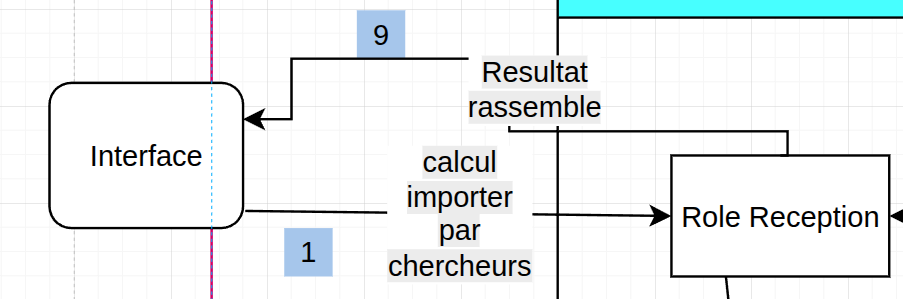
\includegraphics[width=0.5\linewidth]{image.png}
    \caption{Interaction entre le rôle de réception et son environnement}
    \label{fig:interaction_reception_env}
\end{figure}

\begin{figure}[H]
    \centering
    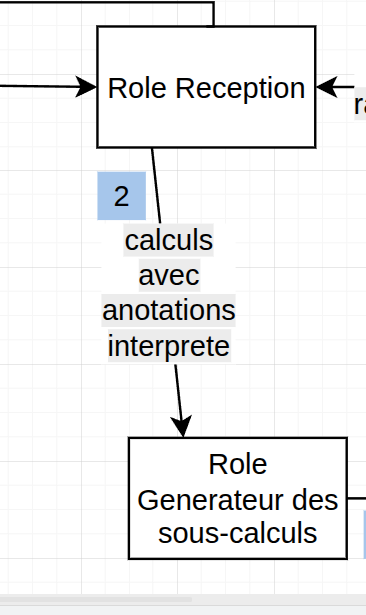
\includegraphics[width=0.5\linewidth]{image2.png}
    \caption{Interaction entre le réceptionniste et le générateur de sous-tâches}
    \label{fig:interaction_reception_generation}
\end{figure}

\begin{figure}[H]
    \centering
    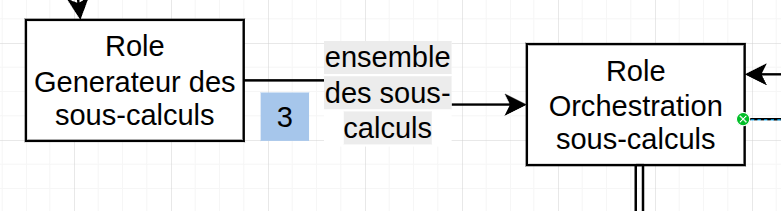
\includegraphics[width=0.5\linewidth]{image3.png}
    \caption{Interaction détaillée entre réception et génération des sous-calculs}
    \label{fig:interaction_detail_generation}
\end{figure}

\begin{figure}[H]
    \centering
    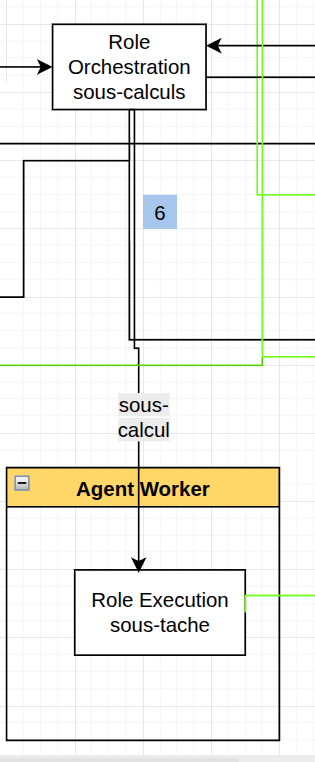
\includegraphics[width=0.5\linewidth]{image4.png}
    \caption{Interaction entre le générateur de sous-calculs et l'orchestrateur}
    \label{fig:interaction_generation_orchestration}
\end{figure}

\begin{figure}[H]
    \centering
    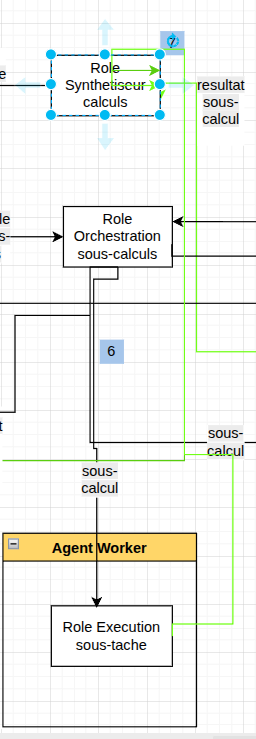
\includegraphics[width=0.5\linewidth]{image5.png}
    \caption{Interaction entre les agents d'exécution et le synthétiseur}
    \label{fig:interaction_execution_synthese}
\end{figure}

\begin{figure}[H]
    \centering
    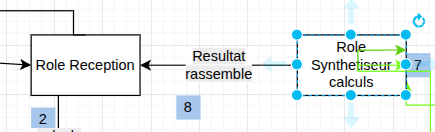
\includegraphics[width=0.5\linewidth]{image6.png}
    \caption{Interaction entre le synthétiseur et le réceptionniste}
    \label{fig:interaction_synthese_reception}
\end{figure}

Les diagrammes de séquences techniques suivants décrivent le comportement détaillé de chaque rôle au niveau de l'implémentation.

\begin{figure}[H]
    \centering
    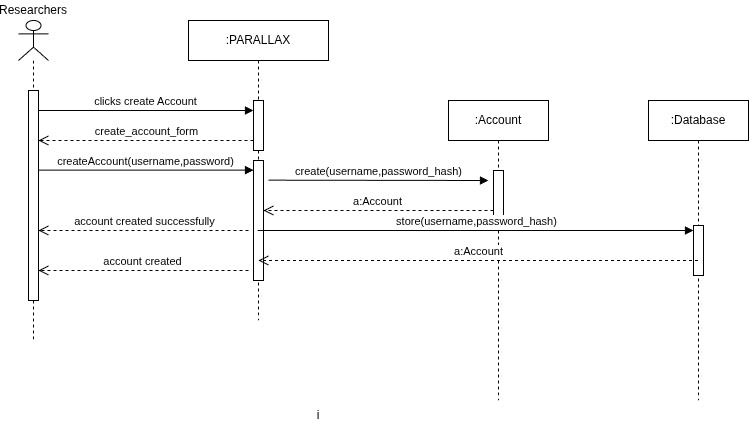
\includegraphics[width=1\textwidth]{images/parallax-AUTHENTIFCATION.jpg.jpeg}
    \caption{Diagramme de séquences technique — Authentification}
    \label{fig:seq_tech_auth}
\end{figure}

\begin{figure}[H]
    \centering
    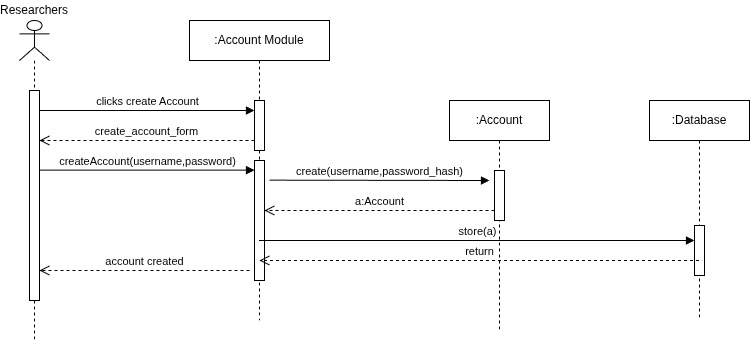
\includegraphics[width=1\textwidth]{images/parallax-CREATE_ACCOUNT.jpg.jpeg}
    \caption{Diagramme de séquences technique — Création de compte}
    \label{fig:seq_tech_account}
\end{figure}

\begin{figure}[H]
    \centering
    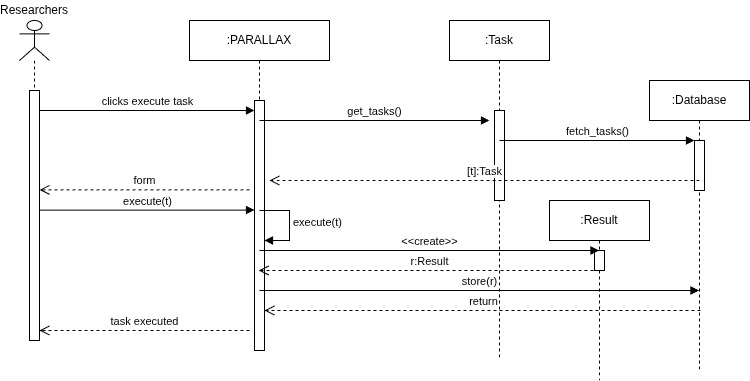
\includegraphics[width=1\textwidth]{images/parallax-ImportTask (2).jpg.jpeg}
    \caption{Diagramme de séquences technique — Importation d'une tâche}
    \label{fig:seq_tech_import}
\end{figure}

\begin{figure}[H]
    \centering
    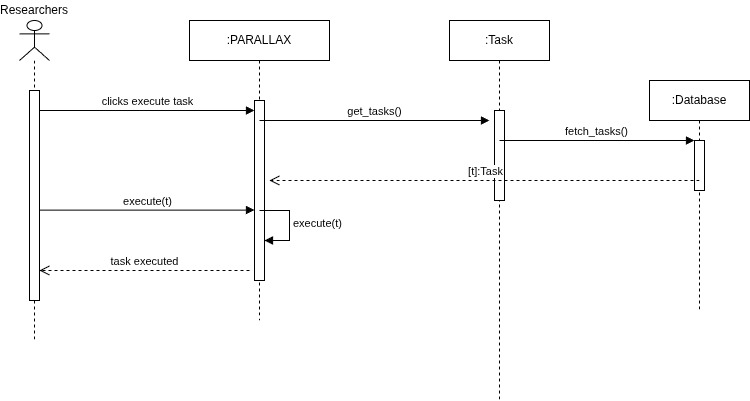
\includegraphics[width=1\textwidth]{images/parallax-ExecuteTask.jpg.jpeg}
    \caption{Diagramme de séquences technique — Exécution d'une tâche}
    \label{fig:seq_tech_execute}
\end{figure}

\begin{figure}[H]
    \centering
    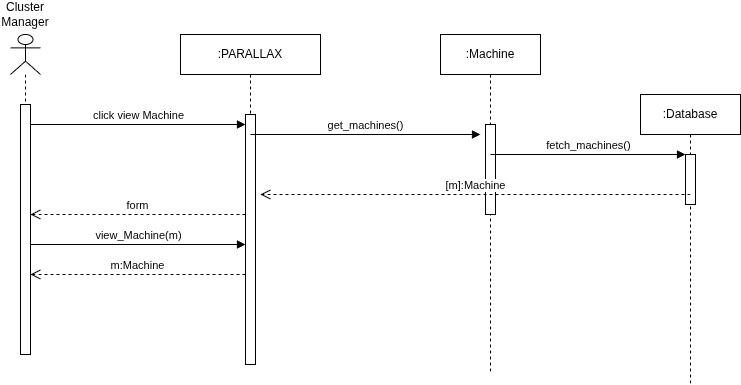
\includegraphics[width=1\textwidth]{images/parallax-consulter_machines (1).jpg.jpeg}
    \caption{Diagramme de séquences technique — Consultation des machines}
    \label{fig:seq_tech_machines}
\end{figure}

\begin{figure}[H]
    \centering
    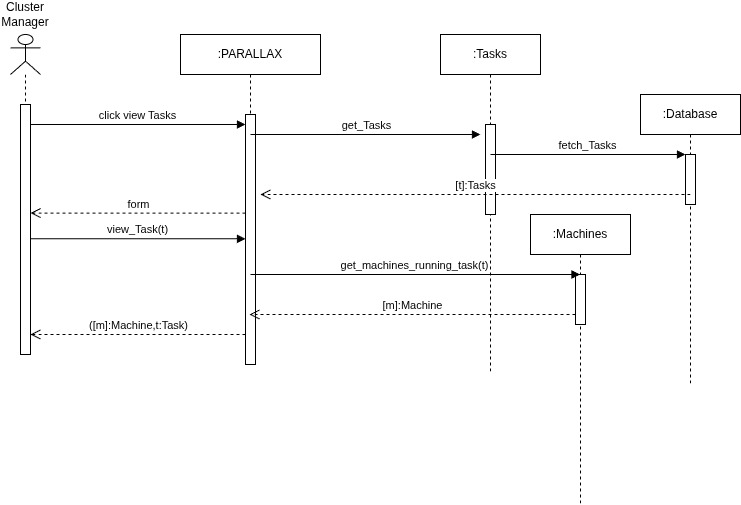
\includegraphics[width=1\textwidth]{images/parallax-consulter_taches (1).jpg.jpeg}
    \caption{Diagramme de séquences technique — Consultation des tâches}
    \label{fig:seq_tech_taches}
\end{figure}

\begin{figure}[H]
    \centering
    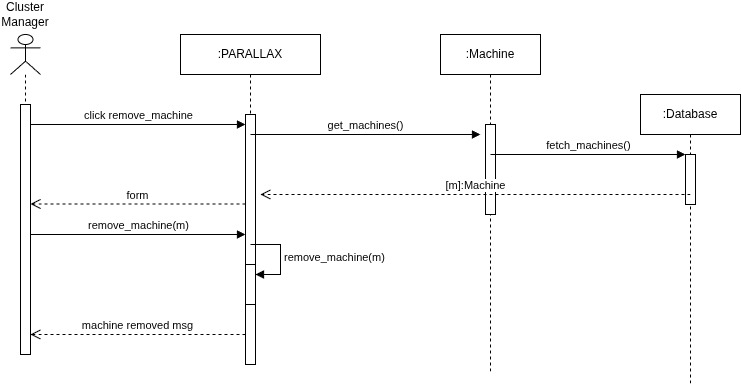
\includegraphics[width=1\textwidth]{images/parallax-Remove_Node.jpg.jpeg}
    \caption{Diagramme de séquences technique — Suppression d'un nœud}
    \label{fig:seq_tech_remove}
\end{figure}

\subsection{Protocoles de communication et coordination}

\subsubsection{Communication inter-agents}

Dans SMA\_PARALLAX, la communication entre agents est \textbf{directe et asynchrone}, reposant sur des messages structurés transportés via TCP sur le réseau local. Chaque message est un acte de communication au sens des ACL : il porte un type d'acte décrivant l'intention de l'émetteur (informer, demander, notifier), un émetteur, un récepteur, un contenu et un identifiant de conversation.

\begin{table}[H]
\centering
\renewcommand{\arraystretch}{1.3}
\begin{tabular}{|l|l|l|l|}
\hline
\textbf{Type d'acte} & \textbf{Acte de communication} & \textbf{Direction} & \textbf{Fonction} \\
\hline
Assertif & \textit{inform} & Worker $\rightarrow$ Contrôleur & Signalement d'état de charge via heartbeat \\
\hline
Directif & \textit{request} & Master $\rightarrow$ Worker & Demande d'exécution d'un sous-calcul \\
\hline
Notification & \textit{notify} & Contrôleur $\rightarrow$ Master & Alerte de défaillance détectée \\
\hline
\end{tabular}
\caption{Types de messages dans SMA\_PARALLAX}
\label{tab:messages_acl}
\end{table}

\paragraph{Structure d'un message de heartbeat}

\[
\mathrm{HB}(i, t) = \big( \mathrm{uuid}_i,\; k_i(t),\; \widehat{\mathrm{CPU}}_i(t),\;
\widehat{\mathrm{RAM}}_i(t),\; q_i(t),\; \mathrm{Score}(i,t),\; \sigma_i,\; L_i(t) \big)
\]

Chaque nœud $n_i$ émet un heartbeat unicast vers le Contrôleur toutes les $T_{\mathrm{HB}} = 2$\,s. Il transporte la télémétrie nécessaire à l'orchestration : charge CPU et RAM, longueur de la file de tâches, score courant et état logique.

\paragraph{Architecture à deux couches}

\textbf{Couche 1 — heartbeat unicast vers le Contrôleur.} Signal périodique de présence et de télémétrie sur le canal best-effort.

\textbf{Couche 2 — gossip inter-pairs.} Toutes les $T_G = 5$\,s, chaque nœud envoie à $k = \lceil \log_2 N \rceil$ pairs aléatoires un résumé de sa vue récente du cluster.

\begin{figure}[H]
\centering
\begin{tikzpicture}[
    leader/.style={circle, draw=red!70!black, thick, minimum size=1.3cm,
                   fill=red!15, font=\bfseries},
    worker/.style={circle, draw=blue!70!black, thick, minimum size=1.1cm, fill=blue!10},
    hb/.style={->, thick, red!60!black},
    gossip/.style={dashed, thick, blue!50}
]
\node[leader] (L) at (0,0) {C};
\node[worker] (W1) at (90:3)   {$W_1$};
\node[worker] (W2) at (30:3)   {$W_2$};
\node[worker] (W3) at (-30:3)  {$W_3$};
\node[worker] (W4) at (-90:3)  {$W_4$};
\node[worker] (W5) at (-150:3) {$W_5$};
\node[worker] (W6) at (150:3)  {$W_6$};
\draw[hb] (W1) -- (L); \draw[hb] (W2) -- (L); \draw[hb] (W3) -- (L);
\draw[hb] (W4) -- (L); \draw[hb] (W5) -- (L); \draw[hb] (W6) -- (L);
\draw[gossip] (W1) to[bend left=15]  (W3);
\draw[gossip] (W2) to[bend right=20] (W5);
\draw[gossip] (W3) to[bend right=15] (W6);
\draw[gossip] (W4) to[bend left=20]  (W1);
\draw[gossip] (W5) to[bend left=15]  (W3);
\draw[gossip] (W6) to[bend right=20] (W4);
\begin{scope}[shift={(5.5,0)}]
    \node[font=\bfseries, anchor=west] at (0,1.5) {Légende};
    \draw[hb]     (0,1)   -- (1.2,1);   \node[anchor=west, font=\small] at (1.3,1)   {HB couche 1};
    \draw[gossip] (0,0.4) -- (1.2,0.4); \node[anchor=west, font=\small] at (1.3,0.4) {Gossip couche 2};
    \node[leader, minimum size=0.7cm, font=\small] at (0.2,-0.4) {C};
    \node[anchor=west, font=\small] at (1.3,-0.4) {Contrôleur};
    \node[worker, minimum size=0.7cm, font=\small] at (0.2,-1.2) {$W$};
    \node[anchor=west, font=\small] at (1.3,-1.2) {Worker};
\end{scope}
\end{tikzpicture}
\caption{Architecture à deux couches du heartbeat}
\label{fig:hb_2layers}
\end{figure}

\subsubsection{Coordination distribuée : élection du nœud remplaçant}

\paragraph{Objectif et déclencheurs}

Le protocole d'élection garantit la présence permanente d'un nœud \textbf{remplaçant} capable d'assurer la continuité en cas de défaillance d'un rôle critique. Trois événements déclenchent une élection :

\begin{itemize}
    \item[$\bullet$] \textbf{(D1) Démarrage à froid :} aucun remplaçant n'est présent dans le cluster.
    \item[$\bullet$] \textbf{(D2) Remplacement de rôle critique :} le Master ou le Contrôleur tombe en panne.
    \item[$\bullet$] \textbf{(D3) Stepdown du remplaçant :} maintenance, surcharge persistante ou réorganisation.
\end{itemize}

\paragraph{Fonction de score}

\[
score(n_i) =
a \cdot \frac{CPU_{libre} \cdot CPU_{total}}{CPU_{libre}^{max} \cdot CPU_{total}^{max}}
+ b \cdot \frac{RAM_{libre} \cdot RAM_{total}}{RAM_{libre}^{max} \cdot RAM_{total}^{max}}
+ c \cdot \frac{LATENCE_{min}}{LATENCE_i}
+ d \cdot \frac{freq_i}{freq_{max}}
\]

avec $a = 0{,}35$, $b = 0{,}35$, $c = 0{,}15$, $d = 0{,}15$.

\begin{algorithm}[H]
\caption{Initiation d'une élection par le nœud $k$}
\begin{algorithmic}[1]
\State $\sigma_k \gets electing$
\State $H \gets \{ j \in V \mid Score_{j,t} > Score_{k,t} \}$
\If{$H = \emptyset$}
    \State diffuser $coord(uuid_k)$
    \State $\sigma_k \gets leader$
\Else
    \ForAll{$j \in H$}
        \State envoyer $election(Score_{k,t}, uuid_k)$ à $j$
    \EndFor
    \State armer temporisation $T_{attente}$
\EndIf
\end{algorithmic}
\end{algorithm}

\begin{algorithm}[H]
\caption{Traitement des messages d'élection}
\begin{algorithmic}[1]
\Procedure{OnReceiveElection}{$s, u$}
    \If{$Score_{k,t} > s$ \textbf{ou} ($Score_{k,t} = s$ \textbf{et} $uuid_k > u$)}
        \State envoyer $alive$ à l'émetteur
        \State \Call{InitiateElection}{$k$}
    \EndIf
\EndProcedure
\Procedure{OnReceiveCoord}{$u$}
    \State $leader_k \gets u$
    \State $\sigma_k \gets normal$
\EndProcedure
\end{algorithmic}
\end{algorithm}

\subsubsection{Coordination distribuée : détection de panne}

\textbf{Phase 1 — Suspicion.} Si $\Delta_{ij}(t) \geq T_{\mathrm{suspect}}$, le nœud $i$ marque $j$ comme \textsc{suspected} et émet un \textsc{gossip\_query} à ses $k$ voisins.

\textbf{Phase 2 — Défaillance confirmée.} Si $\Delta_{ij}(t) \geq T_{\mathrm{failed}}$ et si la majorité des réponses sont négatives, $i$ marque $j$ comme \textsc{failed} et déclenche une élection si $j$ était le Master.

\begin{figure}[H]
\centering
\begin{tikzpicture}[
    ->, >=Latex, thick,
    node_state/.style={circle, draw=black!70, thick, minimum size=1.8cm, align=center}
]
\node[node_state, fill=green!15]  (A) at (0,0)  {\textsc{alive}};
\node[node_state, fill=yellow!25] (S) at (5,0)  {\textsc{suspected}};
\node[node_state, fill=red!15]    (F) at (10,0) {\textsc{failed}};
\draw (A) to[bend left=25]
    node[above, font=\small, align=center]
    {$\Delta_{ij} \geq T_{\mathrm{suspect}}$\\émettre \textsc{gossip\_query}} (S);
\draw (S) to[bend left=25]
    node[below, font=\small, align=center]
    {HB reçu\\\textbf{ou} gossip positif} (A);
\draw (S) to[bend left=25]
    node[above, font=\small, align=center]
    {$\Delta_{ij} \geq T_{\mathrm{failed}}$\\\textbf{et} $|R_{\mathrm{neg}}| \geq \lceil k/2 \rceil$} (F);
\draw (F) to[bend left=50]
    node[below, font=\small] {HB reçu (récupération)} (A);
\draw (A) to[loop above] node[above, font=\small] {HB reçu} (A);
\end{tikzpicture}
\caption{Machine à états — suivi d'un pair par un observateur}
\label{fig:fsm_panne}
\end{figure}

\subsubsection{Coopération dans l'exécution}

\paragraph{Inscription d'un nœud}

\begin{algorithm}[H]
\caption{Entrée d'un nœud dans le réseau}
\label{alg:node_join}
\begin{algorithmic}[1]
\State $N.ip \gets \textsc{DHCP\_REQUEST}()$
\State $N.uuid \gets \textsc{GENERATE\_UUID}()$
\State \textsc{STORE\_LOCAL}($N.uuid$)
\State \textsc{SEND\_BROADCAST}(\texttt{HELLO}, $N.uuid$, $N.ip$)
\If{le Contrôleur reçoit \texttt{HELLO}}
    \State \textsc{REGISTER\_NODE}($N.uuid$, $N.ip$)
    \State \textsc{SEND\_ACK}($N.uuid$)
\EndIf
\State \textsc{CONNECT}($N$, \textsc{CONTROLLER})
\end{algorithmic}
\end{algorithm}

\paragraph{Décomposition et distribution des calculs}

\begin{algorithm}[H]
\caption{Processus de décomposition}
\label{alg:decomposition}
\begin{algorithmic}[1]
\State Parser le programme et remplacer les annotations par les fonctions auxiliaires
\State Exécuter séquentiellement les sections non distribuées
\For{chaque section $S$ distribuée}
    \State Interroger le Contrôleur pour l'état des nœuds disponibles
    \State Calculer la répartition : $w_i = x_i / \sum_{j} x_j$
    \State Envoyer le programme instrumenté aux Workers sélectionnés
    \State Envoyer à chaque Worker le couple $(annotation\_id, data)$
\EndFor
\State Attendre tous les résultats (futex ou équivalent)
\end{algorithmic}
\end{algorithm}

\paragraph{Recomposition des résultats}

\begin{algorithm}[H]
\caption{Processus de recomposition}
\label{alg:recomposition}
\begin{algorithmic}[1]
\State Réceptionner les résultats partiels des Workers
\State Mettre à jour le compteur de complétion via futex
\If{tous les résultats attendus sont reçus}
    \State Appliquer la fonction \texttt{aggregate} définie par l'utilisateur
    \State Combiner les résultats partiels pour produire le résultat global
\Else
    \State Attendre les résultats manquants
\EndIf
\end{algorithmic}
\end{algorithm}

\begin{figure}[H]
    \centering
    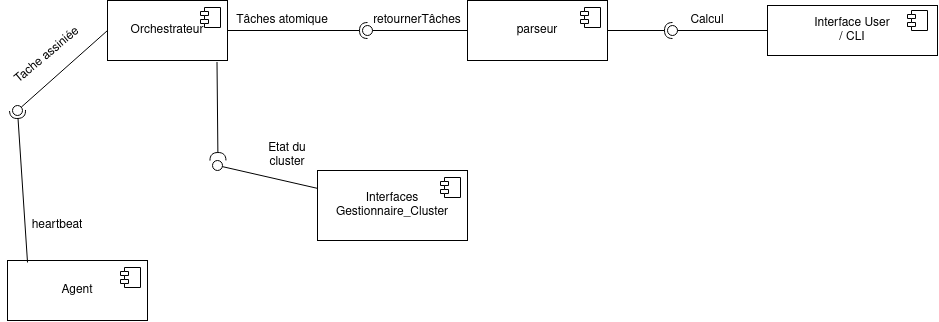
\includegraphics[width=1\textwidth]{images/Diagram des composants - parallax.drawio.png}
    \caption{Diagramme des composants}
    \label{fig:composants}
\end{figure}

% ==============================================================================

\chapter{Implémentation et Résultats}

\section{Conception et limites du modèle réseau classique (Network Agent Abstraction)}

Dans le cadre d'un système multi-agents concurrent comme PARALLAX, l'implémentation de la communication réseau directe au sein de chaque thread applicatif pose des limites physiques et logicielles majeures :
\begin{itemize}
    \item \textbf{Concurrence de binding} : Lorsque plusieurs threads tentent d'écouter ou d'initier des connexions sur la même interface réseau en utilisant des ports spécifiques, des conflits d'allocation d'adresses (erreur \texttt{EADDRINUSE}) surviennent inévitablement.
    \item \textbf{Mélange de flux d'entrée (Stream Mixing)} : Si plusieurs threads accèdent simultanément au même descripteur de socket sans synchronisation rigoureuse, les paquets TCP entrants sont entrelacés. Cela corrompt la sémantique des messages et rend leur désérialisation impossible.
    \item \textbf{Épuisement des ports} : La création et la destruction incessantes de sockets TCP par des threads à durée de vie courte sature la table des descripteurs système et la table de routage (sockets bloqués en état \texttt{TIME\_WAIT}).
\end{itemize}

Pour surmonter ces contraintes, l'architecture de PARALLAX introduit une \textbf{Abstraction d'Agent Réseau} (\texttt{network\_agent.c}). Chaque nœud physique exécute une unique instance d'Agent Réseau persistant qui centralise et orchestre toutes les communications physiques via trois threads spécialisés :
\begin{enumerate}
    \item \texttt{socket\_listener} (TCP) : Un thread d'écoute centralisé sur un port fixe (par exemple 9008 pour le Réceptionniste, 9005 pour le Master, 9006 pour le Worker, 9000 pour le Contrôleur). Il accepte les connexions TCP entrantes de manière asynchrone et les distribue.
    \item \texttt{socket\_sender} (TCP) : Un thread d'expédition unique qui consomme les messages réseau sortants et gère leur transmission physique sans interférence.
    \item \texttt{udp\_socket\_listener} : Dédié à la réception des signaux UDP (notamment pour la découverte dynamique).
\end{enumerate}

Le découplage entre les threads applicatifs et l'Agent Réseau est matérialisé par des \textbf{files de messages IPC System V} (implémentées dans \texttt{ms\_queue.c}). Lorsqu'un thread applicatif souhaite envoyer un message réseau, il pousse un message typé dans la file IPC locale dédiée à l'Agent Réseau (\texttt{outgoing}). Inversement, l'Agent Réseau place les messages entrants dans les files IPC locales spécifiques aux types de messages applicatifs (ex. \texttt{PROG}, \texttt{HELLO}, \texttt{NODES}). Ce mécanisme asynchrone offre un tampon robuste qui élimine toute contention sur les ports réseau physiques.

\section{L'Agent Réceptionniste}

L'Agent Réceptionniste est la passerelle d'accès utilisateur au cluster. Ses responsabilités incluent l'exposition d'endpoints d'administration HTTP, la collecte des logs d'exécution transférés par le Contrôleur et la gestion de son cycle de vie autonome.

\subsection{Architecture multi-thread de l'Agent Réceptionniste}

L'Agent Réceptionniste repose sur l'exécution concurrente de 8 threads, décrits ci-dessous :
\begin{enumerate}
    \item \textbf{Thread Principal} : Initialise le gestionnaire de files de messages IPC, démarre l'Agent Réseau sur le port 9008, crée la file locale \texttt{receptionist\_out} et orchestre la découverte initiale.
    \item \textbf{TCP Listener (Agent Réseau)} : Écoute sur le port 9008 pour recevoir les paquets TCP entrants (mises à jour d'IP, acquittements, logs) et les pousse dans la file IPC.
    \item \textbf{TCP Sender (Agent Réseau)} : Dépile les messages de la file IPC locale et les envoie sur le réseau TCP.
    \item \textbf{UDP Listener (Agent Réseau)} : Écoute sur le port 9009 pour recevoir les réponses UDP.
    \item \textbf{HTTP Server} (\texttt{code\_submission\_listener\_thread}) : Serveur HTTP léger écoutant sur le port 9010. Il expose les routes REST suivantes :
        \begin{itemize}
            \item \texttt{/nodes} : Renvoie la liste et l'état des machines physiques du cluster.
            \item \texttt{/node-logs/<uuid>} : Expose le journal système d'un nœud spécifique.
            \item \texttt{/logs} : Renvoie l'historique global.
            \item Soumission de code : Route POST acceptant le chargement de code source C.
        \end{itemize}
    \item \textbf{Query Master IP} (\texttt{receptionist\_thread}) : Interroge le Contrôleur toutes les 5 secondes via un message \texttt{REQUEST\_MASTER\_IP\_TYPE} pour obtenir l'IP du Master actif en cours, maintenant l'état interne de l'agent à jour.
    \item \textbf{Log Receiver} (\texttt{log\_receiver\_thread}) : Lit les messages de type \texttt{PROG\_LOG\_TYPE} sur la file IPC System V et les écrit de manière persistante sur disque dans des fichiers sous le répertoire \texttt{logs/}.
    \item \textbf{Heartbeat} (\texttt{receptionist\_heartbeat\_thread}) : Émet périodiquement toutes les 2 secondes un paquet de présence de rôle 4 (\texttt{ROLE\_RECEPTIONIST}) à destination du Contrôleur.
\end{enumerate}

La figure \ref{fig:threads_receptionist} modélise l'architecture de ces threads concourants.

\begin{figure}[H]
\centering
\begin{tikzpicture}[
    node distance=1.2cm and 0.8cm,
    thread/.style={rectangle, draw=blue!70!black, fill=blue!10, thick, rounded corners, minimum width=2.8cm, minimum height=0.7cm, align=center, font=\scriptsize},
    ipc/.style={cylinder, draw=red!70!black, fill=red!10, shape border rotate=90, minimum width=1cm, minimum height=0.8cm, align=center, font=\scriptsize},
    net/.style={ellipse, draw=green!70!black, fill=green!10, thick, minimum width=1.5cm, minimum height=0.6cm, align=center, font=\scriptsize}
]
\node[thread] (main) {Thread Principal};
\node[thread, below=of main] (http) {HTTP Listener (9010)};
\node[thread, left=of http] (query) {Query Master IP};
\node[thread, right=of http] (log) {Log Receiver};
\node[thread, below=of http] (hb) {Heartbeat (2s)};
\node[ipc, below=of hb] (mq) {System V IPC\\(receptionist\_out)};
\node[thread, below=of mq] (sender) {TCP Sender};
\node[thread, left=of sender] (listener) {TCP Listener (9008)};
\node[thread, right=of sender] (udp) {UDP Listener (9009)};

\draw[<->, thick] (main) -- (http);
\draw[->, thick] (http) -- (mq);
\draw[->, thick] (query) -- (mq);
\draw[->, thick] (log) -- (mq);
\draw[->, thick] (hb) -- (mq);
\draw[<->, thick] (mq) -- (sender);
\end{tikzpicture}
\caption{Structure des threads de l'Agent Réceptionniste}
\label{fig:threads_receptionist}
\end{figure}

\subsection{Cycle de vie et découverte de l'Agent Réceptionniste}

Lors du démarrage, l'agent génère un identifiant unique (UUID) persistant en lisant la source d'entropie système \texttt{/dev/urandom}, puis stocke cette valeur localement dans le fichier \texttt{.receptionist\_uuid}. 

L'agent entre ensuite dans une phase de découverte UDP active (\texttt{discover\_controller}) : il envoie un message broadcast \texttt{MSG\_HELLO} contenant son UUID et son port réseau local (port 9008) sur le port UDP 9001. Le Contrôleur intercepte ce message, enregistre le Réceptionniste et lui répond directement par une trame UDP unicast de type \texttt{HELLO\_TYPE} contenant la chaîne \texttt{IP:<controller\_ip>} vers le port 9009. Dès réception, l'agent enregistre l'IP du Contrôleur et démarre ses threads fonctionnels.

\begin{figure}[H]
\centering
\begin{tikzpicture}[
    node distance=1.5cm,
    scale=0.9, every node/.style={scale=0.9},
    actor/.style={rectangle, draw=blue!70!black, fill=blue!10, thick, minimum width=2.5cm, minimum height=0.8cm, align=center, font=\small},
    lifeline/.style={thick, dashed, draw=gray},
    message/.style={->, >=stealth, thick, draw=black},
    reply/.style={->, >=stealth, thick, dashed, draw=black},
    active/.style={rectangle, fill=blue!20, draw=blue!70!black, minimum width=0.3cm}
]
% Nodes
\node[actor] (rec) {Réceptionniste};
\node[actor, right=4cm of rec] (ctrl) {Contrôleur};

% Lifelines
\draw[lifeline] (rec.south) -- +(0, -4.0cm) coordinate (rec_bot);
\draw[lifeline] (ctrl.south) -- +(0, -4.0cm) coordinate (ctrl_bot);

% Active regions
\node[active, below=0.3cm of rec.south, minimum height=3.0cm] (rec_act) {};
\node[active, below=0.6cm of ctrl.south, minimum height=2.0cm] (ctrl_act) {};

% Messages
\draw[message] ($(rec_act.north)+(0.15,-0.2)$) -- node[above, font=\scriptsize] {UDP Broadcast \texttt{MSG\_HELLO} (port 9001)} ($(ctrl_act.north)+(-0.15,-0.2)$);
\draw[reply] ($(ctrl_act.north)+(-0.15,-1.2)$) -- node[above, font=\scriptsize] {UDP Unicast \texttt{HELLO\_TYPE} (port 9009)} ($(rec_act.north)+(0.15,-1.2)$);
\draw[message] ($(rec_act.north)+(0.15,-2.2)$) -- node[above, font=\scriptsize, align=center] {Enregistrement IP du Contrôleur\\et activation des threads} ($(rec_act.north)+(0.15,-2.7)$);

\end{tikzpicture}
\caption{Diagramme de séquence : Protocole de découverte de l'Agent Réceptionniste}
\label{fig:seq_discovery}
\end{figure}

\section{L'Agent Master}

L'Agent Master est le coordinateur des calculs. Il centralise les soumissions de code, découpe les tâches, interroge le contrôleur pour localiser les ressources, distribue les sous-calculs et fusionne les résultats.

\subsection{Architecture multi-thread de l'Agent Master}

L'Agent Master structure son exécution autour d'un ensemble de threads concurrents :
\begin{itemize}
    \item \textbf{Thread Principal} : Lance l'Agent Réseau sur le port 9005 et initialise le gestionnaire d'exécutions.
    \item \textbf{Threads de l'Agent Réseau} (\texttt{socket\_listener}, \texttt{socket\_sender}, \texttt{udp\_socket\_listener}).
    \item \textbf{Prog Listener} (\texttt{master\_thread\_start}) : Écoute les nouveaux programmes sur la file de messages IPC locale \texttt{PROG}. À chaque réception, il instancie un thread d'orchestration dédié (\texttt{prog\_listener\_func}) pour compiler et exécuter le code de façon non bloquante.
    \item \textbf{Pool Parallax Team} : Pool dynamique de threads créés par l'orchestrateur. Chaque thread du pool pilote et surveille un Worker distant spécifique pour une tâche donnée.
\end{itemize}

\begin{figure}[H]
\centering
\begin{tikzpicture}[
    node distance=1.2cm and 0.8cm,
    thread/.style={rectangle, draw=blue!70!black, fill=blue!10, thick, rounded corners, minimum width=2.8cm, minimum height=0.7cm, align=center, font=\scriptsize},
    ipc/.style={cylinder, draw=red!70!black, fill=red!10, shape border rotate=90, minimum width=1cm, minimum height=0.8cm, align=center, font=\scriptsize},
    team/.style={rectangle, draw=orange!70!black, fill=orange!10, thick, dashed, rounded corners, minimum width=2.8cm, minimum height=0.7cm, align=center, font=\scriptsize}
]
\node[thread] (main) {Thread Principal};
\node[thread, below=of main] (listener) {Prog Listener (file PROG)};
\node[ipc, below=of listener] (mq) {System V IPC\\(master\_out)};
\node[thread, left=of mq] (net_in) {TCP Listener (9005)};
\node[thread, right=of mq] (net_out) {TCP Sender};
\node[team, below=of mq] (team) {Pool Parallax Team\\(Threads $W_1 \dots W_n$)};

\draw[->, thick] (main) -- (listener);
\draw[->, thick] (listener) -- (team);
\draw[<->, thick] (team) -- (mq);
\draw[->, thick] (net_in) -- (mq);
\draw[->, thick] (mq) -- (net_out);
\end{tikzpicture}
\caption{Structure des threads de l'Agent Master}
\label{fig:threads_master}
\end{figure}

\subsection{Workflow complet d'Orchestration et d'Exécution}

Lorsqu'un programme est reçu, le Master exécute les phases suivantes de manière séquentielle (voir Figure \ref{fig:master_workflow}) :

\begin{enumerate}
    \item \textbf{Parsing du code source} : Le code source C est analysé par le parseur C++ de PARALLAX (\texttt{Parser/build/mytool}). Celui-ci génère un code intermédiaire annoté (\texttt{\_parsed.c}) où les directives de parallélisme sont traduites en structures C standard.
    \item \textbf{Interrogation du Contrôleur} : Le Master émet une requête réseau de type \texttt{NODES} sur le port 9000 du Contrôleur et suspend son exécution sur une file IPC locale temporaire (\texttt{nodes\_mq\_name}). Le Contrôleur renvoie un tableau de structures \texttt{MachineMetrics} de tous les Workers actifs.
    \item \textbf{Tri par Score de Performance} : Le Master trie les Workers disponibles par ordre décroissant de score de performance. La fonction de score d'un nœud $n_i$ est calculée par le Contrôleur et partagée via sa télémétrie :
        \begin{equation}
            \text{score}(n_i) = \alpha \cdot \text{norm\_cpu}_i + \beta \cdot \text{norm\_ram}_i + \gamma \cdot \text{norm\_net}_i + \delta \cdot c\text{\_queue}_i
        \end{equation}
        Où les coefficients de pondération réels sont définis par $\alpha = 0.5$, $\beta = 0.3$, $\gamma = 0.1$, $\delta = 0.1$, et les composantes de capacité sont :
        \begin{itemize}
            \item Capacité de calcul CPU : $C_{\text{cpu}} = \text{cores} \times \text{threads} \times \text{freq\_mhz} \times (1 - \text{cpu\_usage}/100) \times \frac{1}{1 + \text{load1m}}$
            \item Capacité RAM disponible : $C_{\text{ram}} = \text{mem\_available\_mb}$
            \item Capacité réseau : $C_{\text{net}} = \text{network\_bandwidth\_mbps}$
            \item Capacité de file d'attente locale : $c_{\text{queue}} = \frac{1}{1 + \text{queue\_len}}$
        \end{itemize}
        Les valeurs $\text{norm\_X}_i$ représentent la normalisation de la capacité par rapport au maximum observé dans le cluster : $\text{norm\_X}_i = \frac{C_X(i)}{\max_{j} C_X(j)}$. Si un nœud est marqué comme surchargé (\texttt{is\_overloaded}), son score est forcé à $0.0$.
    \item \textbf{Distribution des sous-calculs (SCATTER)} : Le Master segmente le paramètre d'entrée marqué \texttt{PARALLAX\_SCATTER} proportionnellement aux poids de performance calculés des nœuds sélectionnés. Il génère les structures d'assignation \texttt{task\_assignment}.
    \item \textbf{Initialisation de la Parallax Team} : Le Master alloue une structure \texttt{team} contenant une barrière de synchronisation basée sur les verrous de bas niveau Linux (\textbf{futex}) et lance un thread par Worker.
    \item \textbf{Handshake de Communication à 3 étapes} :
        Chaque thread de la team gère la liaison avec son Worker via le protocole suivant :
        \begin{itemize}
            \item \textbf{CHCK} : Envoi d'une requête demandant si le binaire du programme est déjà compilé sur le Worker.
            \item \textbf{PROG} : Si le Worker répond \texttt{NONE}, le Master lui envoie le code source complet à compiler.
            \item \textbf{TASK} : Envoi de la tâche contenant le nom de la fonction à exécuter et le bloc de paramètres d'entrée sérialisés. Le thread bloque en attente de la réponse réseau.
        \end{itemize}
    \item \textbf{Barrière de Synchronisation} : Après avoir reçu son résultat partiel, chaque thread se bloque sur \texttt{barrier\_wait} (synchronisation par futex).
    \item \textbf{Réduction et Agrégation} : Une fois tous les threads libérés, le thread principal applique la fonction de réduction dynamique (par exemple \texttt{sum\_reduce}) sur l'accumulateur des résultats partiels pour générer le résultat consolidé.
    \item \textbf{Shipment des logs} : Le Master récupère le fichier de log local, l'encapsule dans un paquet de type \texttt{PROG\_LOG\_TYPE} et l'envoie au Contrôleur pour archivage.
\end{enumerate}

\begin{figure}[H]
\centering
\begin{tikzpicture}[
    node distance=1.1cm,
    startstop/.style={draw, rectangle, rounded corners, minimum width=3cm, minimum height=0.7cm, align=center, fill=red!15, font=\small},
    process/.style={draw, rectangle, minimum width=3.5cm, minimum height=0.7cm, align=center, fill=orange!15, font=\small},
    decision/.style={draw, diamond, aspect=2, minimum width=3cm, minimum height=0.8cm, align=center, fill=green!15, font=\small},
    arrow/.style={thick,->,>=stealth}
]
\node[startstop] (start) {Début : Code soumis};
\node[process, below=of start] (parse) {Parsing et compilation locale\\(génération de \texttt{\_parsed.c})};
\node[process, below=of parse] (query) {Requête NODES au Contrôleur};
\node[process, below=of query] (score) {Calcul des scores et tri des Workers};
\node[process, below=of score] (team) {Initialisation de la Parallax Team};
\node[decision, below=of team] (chck) {CHCK : Programme\\présent sur Worker?};
\node[process, below=of chck, yshift=-0.5cm] (task) {TASK : Envoi des blocs SCATTER};
\node[process, right=of chck, xshift=1.5cm] (prog) {PROG : Transfert du code};
\node[process, below=of task] (barrier) {Barrière futex (attente résultats)};
\node[process, below=of barrier] (reduce) {Réduction des résultats (aggregator)};
\node[startstop, below=of reduce] (end) {Fin : Résultat réduit};

\draw [arrow] (start) -- (parse);
\draw [arrow] (parse) -- (query);
\draw [arrow] (query) -- (score);
\draw [arrow] (score) -- (team);
\draw [arrow] (team) -- (chck);
\draw [arrow] (chck) -- node[left] {Oui} (task);
\draw [arrow] (chck) -- node[above] {Non} (prog);
\draw [arrow] (prog) |- (task);
\draw [arrow] (task) -- (barrier);
\draw [arrow] (barrier) -- (reduce);
\draw [arrow] (reduce) -- (end);
\end{tikzpicture}
\caption{Diagramme d'activité : Workflow d'exécution de l'Agent Master}
\label{fig:master_workflow}
\end{figure}

\section{L'Agent Worker}

L'Agent Worker s'exécute sur chaque nœud de calcul du cluster. Il est responsable de la compilation dynamique des tâches, de leur isolation à l'exécution et du contrôle local des ressources.

\subsection{Architecture multi-thread de l'Agent Worker}

L'Agent Worker s'appuie sur les threads concurrents suivants :
\begin{itemize}
    \item \textbf{Thread Principal} : Lance l'Agent Réseau sur le port 9006, crée les files IPC locales et attend les ordres du Master.
    \item \textbf{Agent Réseau} (\texttt{socket\_listener}, \texttt{socket\_sender}, \texttt{udp\_socket\_listener}).
    \item \textbf{Execution Thread} : Traite le protocole CHCK/PROG/TASK de manière séquentielle pour un Master donné.
    \item \textbf{Log Monitor Thread} : Surveille la taille du fichier journal généré par les processus exécutés.
\end{itemize}

\begin{figure}[H]
\centering
\begin{tikzpicture}[
    node distance=1.2cm and 0.8cm,
    thread/.style={rectangle, draw=blue!70!black, fill=blue!10, thick, rounded corners, minimum width=2.8cm, minimum height=0.7cm, align=center, font=\scriptsize},
    ipc/.style={cylinder, draw=red!70!black, fill=red!10, shape border rotate=90, minimum width=1cm, minimum height=0.8cm, align=center, font=\scriptsize}
]
\node[thread] (main) {Thread Principal};
\node[thread, below=of main] (exec) {Execution Thread\\(CHCK/PROG/TASK)};
\node[thread, left=of exec] (log) {Log Monitor Thread};
\node[thread, right=of exec] (hb) {Heartbeat Thread};
\node[ipc, below=of exec] (mq) {System V IPC\\(worker\_out)};
\node[thread, left=of mq] (net_in) {TCP Listener (9006)};
\node[thread, right=of mq] (net_out) {TCP Sender};

\draw[->, thick] (main) -- (exec);
\draw[->, thick] (main) -- (log);
\draw[->, thick] (main) -- (hb);
\draw[->, thick] (exec) -- (mq);
\draw[->, thick] (net_in) -- (mq);
\draw[->, thick] (mq) -- (net_out);
\end{tikzpicture}
\caption{Structure des threads de l'Agent Worker}
\label{fig:threads_worker}
\end{figure}

\subsection{Compilation Dynamique, Isolation et Rotation des Logs}

\paragraph{Compilation dynamique sans main()}
Afin d'exécuter des fonctions spécifiques reçues dynamiquement sans redémarrer le daemon Worker, le code compilé n'intègre pas la fonction traditionnelle \texttt{main()}. Le Worker compile les programmes reçus sous forme de binaires autonomes en injectant le drapeau de liaison GCC \texttt{-Wl,-e,worker\_entry}. Ce drapeau redéfinit le point d'entrée d'exécution au niveau de la fonction \texttt{worker\_entry()}, qui prend en charge la désérialisation locale des paramètres.

\paragraph{Isolation de l'exécution}
Pour empêcher qu'un calcul utilisateur corrompu ne fasse planter le daemon principal du Worker, chaque exécution de tâche est isolée dans un processus séparé :
\begin{enumerate}
    \item Le Worker effectue un appel système \texttt{fork()}.
    \item Le processus fils redirige son flux de sortie standard (stdout/stderr) vers un fichier de log via des descripteurs de fichiers dupliqués (\texttt{dup2()}).
    \item Le fils charge et exécute le binaire compilé de la tâche via un appel système \texttt{execv()}.
    \item Le processus père (le daemon Worker) surveille l'exécution du fils et récupère le code de retour à la fin.
\end{enumerate}

\paragraph{Rotation et surveillance des logs}
Le thread \texttt{Log Monitor} vérifie en tâche de fond la taille du fichier de log associé à l'exécution en cours. Si la taille du fichier dépasse un seuil de \textbf{512 Ko}, le thread tronque le fichier et effectue une rotation pour préserver l'espace disque du nœud de calcul et éviter tout déni de service local.

\section{L'Agent Contrôleur}

L'Agent Contrôleur est le superviseur du cluster. Il centralise les battements de cœur, maintient la table d'état globale des nœuds et détecte les pannes.

\subsection{Architecture multi-thread de l'Agent Contrôleur}

Pour traiter les messages asynchrones du cluster sans blocage, le Contrôleur maintient une structure hautement parallèle comprenant \textbf{15 threads simultanés} :
\begin{itemize}
    \item \textbf{Thread Principal} : Démarre l'Agent Réseau sur le port 9000.
    \item \textbf{Agent Réseau} (\texttt{socket\_listener}, \texttt{socket\_sender}, \texttt{udp\_socket\_listener}).
    \item \textbf{11 Threads de Traitement (Handlers IPC)} :
        \begin{itemize}
            \item \texttt{hello\_func} : Traite les requêtes \texttt{HELLO} UDP, enregistre les nœuds et renvoie l'IP du Contrôleur.
            \item \texttt{heartbeat\_receiver\_func} : Reçoit les pulsations UDP et met à jour l'horodatage de présence.
            \item \texttt{statecapture\_init\_func} : Enregistre les métriques matérielles initiales lors de la première connexion.
            \item \texttt{statecapture\_func} : Met à jour les métriques dynamiques des nœuds (CPU, RAM, bande passante).
            \item \texttt{node\_log\_receiver\_func} : Reçoit les logs système des Workers et les écrit dans \texttt{node\_logs/}.
            \item \texttt{get\_node\_log\_func} : Transmet les logs archivés à la demande de l'Agent Réceptionniste.
            \item \texttt{log\_relay\_func} : Redirige les journaux d'exécution reçus des Masters vers l'Agent Réceptionniste connecté.
            \item \texttt{request\_master\_ip\_func} : Répond aux demandes de l'IP du Master formulées par le Réceptionniste.
            \item Trois threads de maintenance interne et de surveillance périodique.
        \end{itemize}
\end{itemize}

\begin{figure}[H]
\centering
\begin{tikzpicture}[
    node distance=1.2cm and 0.8cm,
    thread/.style={rectangle, draw=blue!70!black, fill=blue!10, thick, rounded corners, minimum width=2.8cm, minimum height=0.7cm, align=center, font=\scriptsize},
    ipc/.style={cylinder, draw=red!70!black, fill=red!10, shape border rotate=90, minimum width=1cm, minimum height=0.8cm, align=center, font=\scriptsize},
    group/.style={rectangle, draw=purple!70!black, fill=purple!5, thick, dotted, rounded corners, minimum width=6cm, minimum height=1.8cm, align=center, font=\scriptsize}
]
\node[thread] (main) {Thread Principal};
\node[group, below=of main] (handlers) {11 Threads de Traitement (Handlers IPC)\\ (statecapture, hello, heartbeat, log\_relay, request\_master\_ip, etc.)};
\node[ipc, below=of handlers] (mq) {System V IPC\\(controller\_out)};
\node[thread, left=of mq] (net_in) {TCP Listener (9000)};
\node[thread, right=of mq] (net_out) {TCP Sender};

\draw[->, thick] (main) -- (handlers);
\draw[<->, thick] (handlers) -- (mq);
\draw[->, thick] (net_in) -- (mq);
\draw[->, thick] (mq) -- (net_out);
\end{tikzpicture}
\caption{Structure des threads de l'Agent Contrôleur}
\label{fig:threads_controller}
\end{figure}

\subsection{Mécanisme de Watchdog et Détection de pannes}

Le Contrôleur exécute périodiquement un algorithme de vérification d'état (Watchdog) sur sa table des nœuds connectés (\texttt{g\_node\_table}). Pour chaque nœud $n_j$, la durée écoulée depuis le dernier heartbeat reçu est calculée : $\Delta_j = t - \text{last\_heartbeat}_j$. 

Les transitions d'état sont appliquées strictement selon les règles temporelles définies en configuration :
\begin{enumerate}
    \item \textbf{Transition en état SUSPECT} : Si $\Delta_j \geq T_{\text{suspect}} = 4$ secondes, le Contrôleur marque le nœud comme \texttt{NODE\_SUSPECT} et initie une requête de confirmation Gossip vers les autres nœuds.
    \item \textbf{Transition en état EN PANNE} : Si $\Delta_j \geq T_{\text{failed}} = 8$ secondes, le Contrôleur confirme la défaillance, bascule l'état du nœud à \texttt{NODE\_EN\_PANNE} et retire le nœud du pool des Workers actifs. Si le nœud en panne était le Master actif du cluster, le Contrôleur initie immédiatement une élection pour désigner un nouveau Master parmi les Workers fonctionnels restants.
\end{enumerate}

\section{Trace complète d'un cycle de calcul}

Le fonctionnement de PARALLAX s'articule autour des 9 étapes suivantes lors d'un calcul utilisateur :

\begin{enumerate}
    \item \textbf{Soumission HTTP} : L'utilisateur soumet son code C annoté (contenant une directive de parallélisme comme un bloc d'exécution parallèle) à l'Agent Réceptionniste via une requête HTTP POST sur le port 9010.
    \item \textbf{Transfert au Master} : Le Réceptionniste interroge le Contrôleur pour obtenir l'IP du Master actif, puis pousse le programme reçu dans la file IPC réseau du Master.
    \item \textbf{Parsing \& Compilation} : Le Master reçoit le programme via son thread \texttt{master\_thread\_start}, le parse en C++ pour générer le code source distribué, et le compile sous forme de binaire de contrôle.
    \item \textbf{Récupération des ressources} : Le Master envoie une requête \texttt{NODES} au Contrôleur et récupère les métriques en temps réel des Workers actifs du cluster.
    \item \textbf{Calcul des scores \& Planification} : Le Master trie les Workers par leur score de performance calculé, décide de la distribution des données du bloc \texttt{SCATTER} et crée la Parallax Team d'exécution.
    \item \textbf{Handshake CHCK-PROG-TASK} : Chaque thread de la team gère la liaison avec son Worker via le protocole suivant :
        \begin{itemize}
            \item \textbf{CHCK} : Envoi d'une requête demandant si le binaire du programme est déjà compilé sur le Worker.
            \item \textbf{PROG} : Si le Worker répond \texttt{NONE}, le Master lui envoie le code source complet à compiler.
            \item \textbf{TASK} : Envoi de la tâche contenant le nom de la fonction à exécuter et le bloc de paramètres d'entrée sérialisés. Le thread bloque en attente de la réponse réseau.
        \end{itemize}
    \item \textbf{Barrière de Synchronisation} : Après avoir reçu son résultat partiel, chaque thread se bloque sur \texttt{barrier\_wait} (synchronisation par futex).
    \item \textbf{Réduction et Agrégation} : Une fois tous les threads libérés, le thread principal applique la fonction de réduction dynamique (par exemple \texttt{sum\_reduce}) sur l'accumulateur des résultats partiels pour générer le résultat consolidé.
    \item \textbf{Shipment des logs} : Le Master récupère le fichier de log local, l'encapsule dans un paquet de type \texttt{PROG\_LOG\_TYPE} et l'envoie au Contrôleur pour archivage.
\end{enumerate}

\begin{figure}[H]
\centering
\begin{tikzpicture}[
    node distance=1.1cm,
    startstop/.style={draw, rectangle, rounded corners, minimum width=3cm, minimum height=0.7cm, align=center, fill=red!15, font=\small},
    process/.style={draw, rectangle, minimum width=3.5cm, minimum height=0.7cm, align=center, fill=orange!15, font=\small},
    decision/.style={draw, diamond, aspect=2, minimum width=3cm, minimum height=0.8cm, align=center, fill=green!15, font=\small},
    arrow/.style={thick,->,>=stealth}
]
\node[startstop] (start) {Début : Code soumis};
\node[process, below=of start] (parse) {Parsing et compilation locale\\(génération de \texttt{\_parsed.c})};
\node[process, below=of parse] (query) {Requête NODES au Contrôleur};
\node[process, below=of query] (score) {Calcul des scores et tri des Workers};
\node[process, below=of score] (team) {Initialisation de la Parallax Team};
\node[decision, below=of team] (chck) {CHCK : Programme\\présent sur Worker?};
\node[process, below=of chck, yshift=-0.5cm] (task) {TASK : Envoi des blocs SCATTER};
\node[process, right=of chck, xshift=1.5cm] (prog) {PROG : Transfert du code};
\node[process, below=of task] (barrier) {Barrière futex (attente résultats)};
\node[process, below=of barrier] (reduce) {Réduction des résultats (aggregator)};
\node[startstop, below=of reduce] (end) {Fin : Résultat réduit};

\draw [arrow] (start) -- (parse);
\draw [arrow] (parse) -- (query);
\draw [arrow] (query) -- (score);
\draw [arrow] (score) -- (team);
\draw [arrow] (team) -- (chck);
\draw [arrow] (chck) -- node[left] {Oui} (task);
\draw [arrow] (chck) -- node[above] {Non} (prog);
\draw [arrow] (prog) |- (task);
\draw [arrow] (task) -- (barrier);
\draw [arrow] (barrier) -- (reduce);
\draw [arrow] (reduce) -- (end);
\end{tikzpicture}
\caption{Diagramme d'activité : Workflow d'exécution de l'Agent Master}
\label{fig:master_workflow}
\end{figure}

\begin{figure}[H]
\centering
\begin{tikzpicture}[
    scale=0.82, every node/.style={scale=0.82},
    actor/.style={rectangle, draw=blue!70!black, fill=blue!10, thick, minimum width=2.0cm, minimum height=0.7cm, align=center, font=\small},
    lifeline/.style={thick, dashed, draw=gray},
    message/.style={->, >=stealth, thick, draw=black},
    reply/.style={->, >=stealth, thick, dashed, draw=black},
    active/.style={rectangle, fill=blue!20, draw=blue!70!black, minimum width=0.25cm}
]
% Nodes
\node[actor] (user) {Utilisateur};
\node[actor, right=2.0cm of user] (rec) {Réceptionniste};
\node[actor, right=2.0cm of rec] (mast) {Master};
\node[actor, right=2.0cm of mast] (ctrl) {Contrôleur};
\node[actor, right=2.0cm of ctrl] (work) {Worker};

% Lifelines
\draw[lifeline] (user.south) -- +(0, -11.0cm) coordinate (user_bot);
\draw[lifeline] (rec.south) -- +(0, -11.0cm) coordinate (rec_bot);
\draw[lifeline] (mast.south) -- +(0, -11.0cm) coordinate (mast_bot);
\draw[lifeline] (ctrl.south) -- +(0, -11.0cm) coordinate (ctrl_bot);
\draw[lifeline] (work.south) -- +(0, -11.0cm) coordinate (work_bot);

% Active regions
\node[active, below=0.5cm of user.south, minimum height=10.0cm] (user_act) {};
\node[active, below=0.5cm of rec.south, minimum height=9.8cm] (rec_act) {};
\node[active, below=1.2cm of mast.south, minimum height=8.0cm] (mast_act) {};
\node[active, below=2.0cm of ctrl.south, minimum height=7.0cm] (ctrl_act) {};
\node[active, below=4.5cm of work.south, minimum height=4.0cm] (work_act) {};

% Messages
\draw[message] ($(user_act.north)+(0.12,-0.2)$) -- node[above, font=\scriptsize] {POST /submit (Code C)} ($(rec_act.north)+(-0.12,-0.2)$);
\draw[message] ($(rec_act.north)+(0.12,-0.5)$) -- node[above, font=\scriptsize] {Query Master IP} ($(ctrl_act.north)+(-0.12,-0.5)$);
\draw[reply] ($(ctrl_act.north)+(-0.12,-0.9)$) -- node[above, font=\scriptsize] {Master IP} ($(rec_act.north)+(0.12,-0.9)$);
\draw[message] ($(rec_act.north)+(0.12,-1.2)$) -- node[above, font=\scriptsize] {Forward Code (IPC)} ($(mast_act.north)+(-0.12,-1.2)$);

% Master orchestration
\draw[message] ($(mast_act.north)+(0.12,-1.8)$) -- node[above, font=\scriptsize] {Request NODES} ($(ctrl_act.north)+(-0.12,-1.8)$);
\draw[reply] ($(ctrl_act.north)+(-0.12,-2.3)$) -- node[above, font=\scriptsize] {Metrics \& Scores} ($(mast_act.north)+(0.12,-2.3)$);

% Handshake
\draw[message] ($(mast_act.north)+(0.12,-3.5)$) -- node[above, font=\scriptsize] {1. CHCK} ($(work_act.north)+(-0.12,-0.2)$);
\draw[reply] ($(work_act.north)+(-0.12,-0.6)$) -- node[above, font=\scriptsize] {NONE} ($(mast_act.north)+(0.12,-4.1)$);
\draw[message] ($(mast_act.north)+(0.12,-4.5)$) -- node[above, font=\scriptsize] {2. PROG (Code)} ($(work_act.north)+(-0.12,-1.2)$);
\draw[reply] ($(work_act.north)+(-0.12,-1.6)$) -- node[above, font=\scriptsize] {OK} ($(mast_act.north)+(0.12,-5.1)$);
\draw[message] ($(mast_act.north)+(0.12,-5.5)$) -- node[above, font=\scriptsize] {3. TASK (Data)} ($(work_act.north)+(-0.12,-2.2)$);

% Worker execution & logs
\draw[message] ($(work_act.north)+(0.12,-2.6)$) -- node[above, font=\scriptsize] {Send Logs} ($(ctrl_act.north)+(0.12,-4.9)$);
\draw[reply] ($(work_act.north)+(-0.12,-3.2)$) -- node[above, font=\scriptsize] {Result Partiel} ($(mast_act.north)+(0.12,-6.7)$);

% Reduction and final output
\draw[reply] ($(mast_act.north)+(-0.12,-7.4)$) -- node[above, font=\scriptsize] {Reduced Result} ($(rec_act.north)+(0.12,-8.0)$);
\draw[reply] ($(rec_act.north)+(-0.12,-8.5)$) -- node[above, font=\scriptsize] {HTTP Response} ($(user_act.north)+(0.12,-8.9)$);

\end{tikzpicture}
\caption{Diagramme de séquence : Interaction globale lors d'un cycle de calcul}
\label{fig:seq_execution}
\end{figure}



\chapter*{Conclusion Générale}
\addcontentsline{toc}{chapter}{Conclusion Générale}

Le projet PARALLAX, réalisé dans le contexte académique de l’École Nationale Supérieure Polytechnique de Yaoundé, a permis de concevoir et de modéliser une infrastructure de calcul distribué basée sur l’exploitation de machines locales hétérogènes et sous-utilisées.

L’approche adoptée, fondée sur les Systèmes Multi-Agents, a facilité la structuration du système en entités autonomes assurant les fonctions de coordination, d’exécution et de supervision. Cette modélisation a contribué à améliorer la résilience du système face aux défaillances et à mieux organiser la répartition des charges dans un environnement distribué.

Les résultats obtenus montrent que l’architecture mise en place permet d’améliorer l’utilisation des ressources disponibles et de réduire les temps d’exécution pour certaines classes de tâches. Le système valide également sa capacité à maintenir son fonctionnement en présence de pannes partielles.

Les perspectives de ce travail incluent l’amélioration des politiques d’ordonnancement, notamment par l’intégration de techniques d’apprentissage automatique afin d’optimiser dynamiquement l’allocation des tâches au sein du cluster.

\section*{Références}
\addcontentsline{toc}{chapter}{Références}

\begin{thebibliography}{99}

\bibitem{seti}
D. P. Anderson, ``SETI@home: An Experiment in Public-Resource Computing,''
\textit{Communications of the ACM}, vol. 45, no. 11, pp. 56--61, 2002.

\bibitem{htcondor}
D. Thain, T. Tannenbaum, and M. Livny,
``Distributed Computing in Practice: The Condor Experience,''
\textit{Concurrency and Computation: Practice and Experience}, vol. 17, no. 2--4, pp. 323--356, 2005.

\bibitem{tanenbaum_ds}
A. S. Tanenbaum and M. Van Steen,
\textit{Distributed Systems: Principles and Paradigms}, 2nd ed. Prentice Hall, 2007.

\bibitem{wooldridge}
M. Wooldridge,
\textit{An Introduction to MultiAgent Systems}. John Wiley \& Sons, 2009.

\bibitem{topcuoglu}
H. Topcuoglu, S. Hariri, and M.-Y. Wu,
``Performance-Effective and Low-Complexity Task Scheduling for Heterogeneous Computing,''
\textit{IEEE Trans. Parallel Distrib. Syst.}, vol. 13, no. 3, pp. 260--274, 2002.

\bibitem{kubernetes}
B. Burns, J. Beda, and K. Hightower,
\textit{Kubernetes: Up and Running}. O'Reilly Media, 2019.

\bibitem{bully}
H. Garcia-Molina,
``Elections in a Distributed Computing System,''
\textit{IEEE Trans. Computers}, vol. C-31, no. 1, pp. 48--59, 1982.

\bibitem{chapitre1}
Cours d'Agents Intelligents et Systèmes Multi-Agents,
\textit{Chapitre 1 : Agents et Systèmes Multi-Agents — Définitions et Caractéristiques},
A. M. Florea, Université Politehnica de Bucarest / ENSPY, 2024.

\bibitem{chapitre2}
Cours d'Agents Intelligents et Systèmes Multi-Agents,
\textit{Chapitre 2 : Typologie des Agents},
ENSPY — Génie Informatique, 2024.

\end{thebibliography}

\section*{Annexes}

\end{document}